\documentclass[12pt]{article}
\usepackage[utf8]{inputenc}
\usepackage[russian]{babel}
\usepackage{amsmath, amssymb}
\usepackage{graphicx}
\usepackage{float}
\usepackage{geometry}
\usepackage{listings}
\usepackage{xcolor}

\geometry{a4paper, left=2cm, right=2cm, top=2cm, bottom=2cm}

\lstset{
    language=Python,
    basicstyle=\small\ttfamily,
    keywordstyle=\color{blue},
    commentstyle=\color{green!50!black},
    stringstyle=\color{red},
    breaklines=true,
    showstringspaces=false,
    frame=single,
    numbers=left,
    numberstyle=\tiny\color{gray},
    captionpos=b
}

\begin{document}

\begin{titlepage}
    \begin{center}
        \vspace*{\fill}
        
        \textbf{\LARGE Отчет по лабораторной работе №2 «Интерполяция алгебраическими многочленами»}
        
        \vspace{0.5cm}
        
        \textbf{\Large  Николаева Ксения, 9 группа}
        
        
        \vfill
        
    \end{center}
\end{titlepage}

\tableofcontents
\newpage

\section{Постановка задачи}

На отрезке $[a, b] = [-3, 3]$ заданы функции:
\begin{align}
    f_1(x) &= x^2\cos(2x)\\
    f_2(x) &= \frac{1}{1 + 5x^2}
\end{align}

Требуется построить интерполяционные многочлены в форме Ньютона степени $n$, интерполирующие каждую из функций:
\begin{enumerate}
    \item на сетке равноотстоящих узлов;
    \item на сетке чебышёвских узлов.
\end{enumerate}

\section{Теоретические сведения}

\subsection{Выбор узлов интерполяции}

В данной работе используются два способа выбора узлов интерполяции:

\subsubsection{Равноотстоящие узлы}

Равноотстоящие узлы на отрезке $[a, b]$ определяются как:
\begin{equation}
    x_i = a + i \cdot \frac{b - a}{n}, \quad i = 0, 1, \ldots, n
\end{equation}

\subsubsection{Чебышёвские узлы}

Чебышёвские узлы на отрезке $[a, b]$ определяются как:
\begin{equation}
    x_i = \frac{a + b}{2} + \frac{b - a}{2} \cdot \cos\left(\frac{\pi(2i+1)}{2(n+1)}\right), \quad i = 0, 1, \ldots, n
\end{equation}

Чебышёвские узлы позволяют минимизировать максимальную погрешность интерполяции за счет оптимального размещения точек интерполяции.

\subsection{Интерполяционный многочлен в форме Ньютона}

Интерполяционный многочлен Ньютона для функции $f(x)$ на узлах $x_0, x_1, \ldots, x_n$ представляется в виде:
\begin{equation}
    P_n(x) = f[x_0] + f[x_0, x_1](x - x_0) + f[x_0, x_1, x_2](x - x_0)(x - x_1) + \ldots + f[x_0, x_1, \ldots, x_n]\prod_{i=0}^{n-1}(x - x_i)
\end{equation}

где $f[x_0, x_1, \ldots, x_k]$ - разделённые разности $k$-го порядка, которые рекурсивно определяются как:
\begin{align}
    f[x_i] &= f(x_i)\\
    f[x_i, x_{i+1}, \ldots, x_{i+k}] &= \frac{f[x_{i+1}, \ldots, x_{i+k}] - f[x_i, \ldots, x_{i+k-1}]}{x_{i+k} - x_i}
\end{align}

\subsection{Схема Горнера}

Для эффективного вычисления значения интерполяционного многочлена Ньютона используется схема Горнера. Если интерполяционный многочлен представлен в форме Ньютона:
\begin{equation}
    P_n(x) = c_0 + c_1(x-x_0) + c_2(x-x_0)(x-x_1) + \ldots + c_n(x-x_0)(x-x_1)\ldots(x-x_{n-1})
\end{equation}

где $c_i = f[x_0, x_1, \ldots, x_i]$, то значение многочлена можно вычислить по следующей схеме:
\begin{align}
    P_n(x) &= c_n \\
    P_n(x) &= P_n(x) \cdot (x - x_{n-i-1}) + c_{n-i-1}, \quad i = 0, 1, \ldots, n-1
\end{align}

Это позволяет снизить вычислительную сложность с $O(n^2)$ до $O(n)$.

\section{Реализация алгоритма}

Для реализации интерполяционных многочленов был разработан алгоритм на языке Python, который включает в себя:

\begin{enumerate}
    \item Функции для генерации равноотстоящих и чебышёвских узлов
    \item Функцию для вычисления разделённых разностей
    \item Функцию для вычисления значения интерполяционного многочлена Ньютона с использованием схемы Горнера
    \item Функции для построения графиков и расчёта погрешностей
\end{enumerate}

Особенностями реализации являются:
\begin{itemize}
    \item Использование одномерных массивов для эффективного хранения данных
    \item Применение схемы Горнера для оптимизации вычислений значений многочлена
    \item Переиспользование узлов интерполяции для обеих функций, что позволяет сократить количество операций
\end{itemize}

\section{Результаты интерполяции для функции $f_1(x) = x^2\cos(2x)$}

\subsection{Графики интерполяционных многочленов}

\begin{figure}[H]
    \centering
    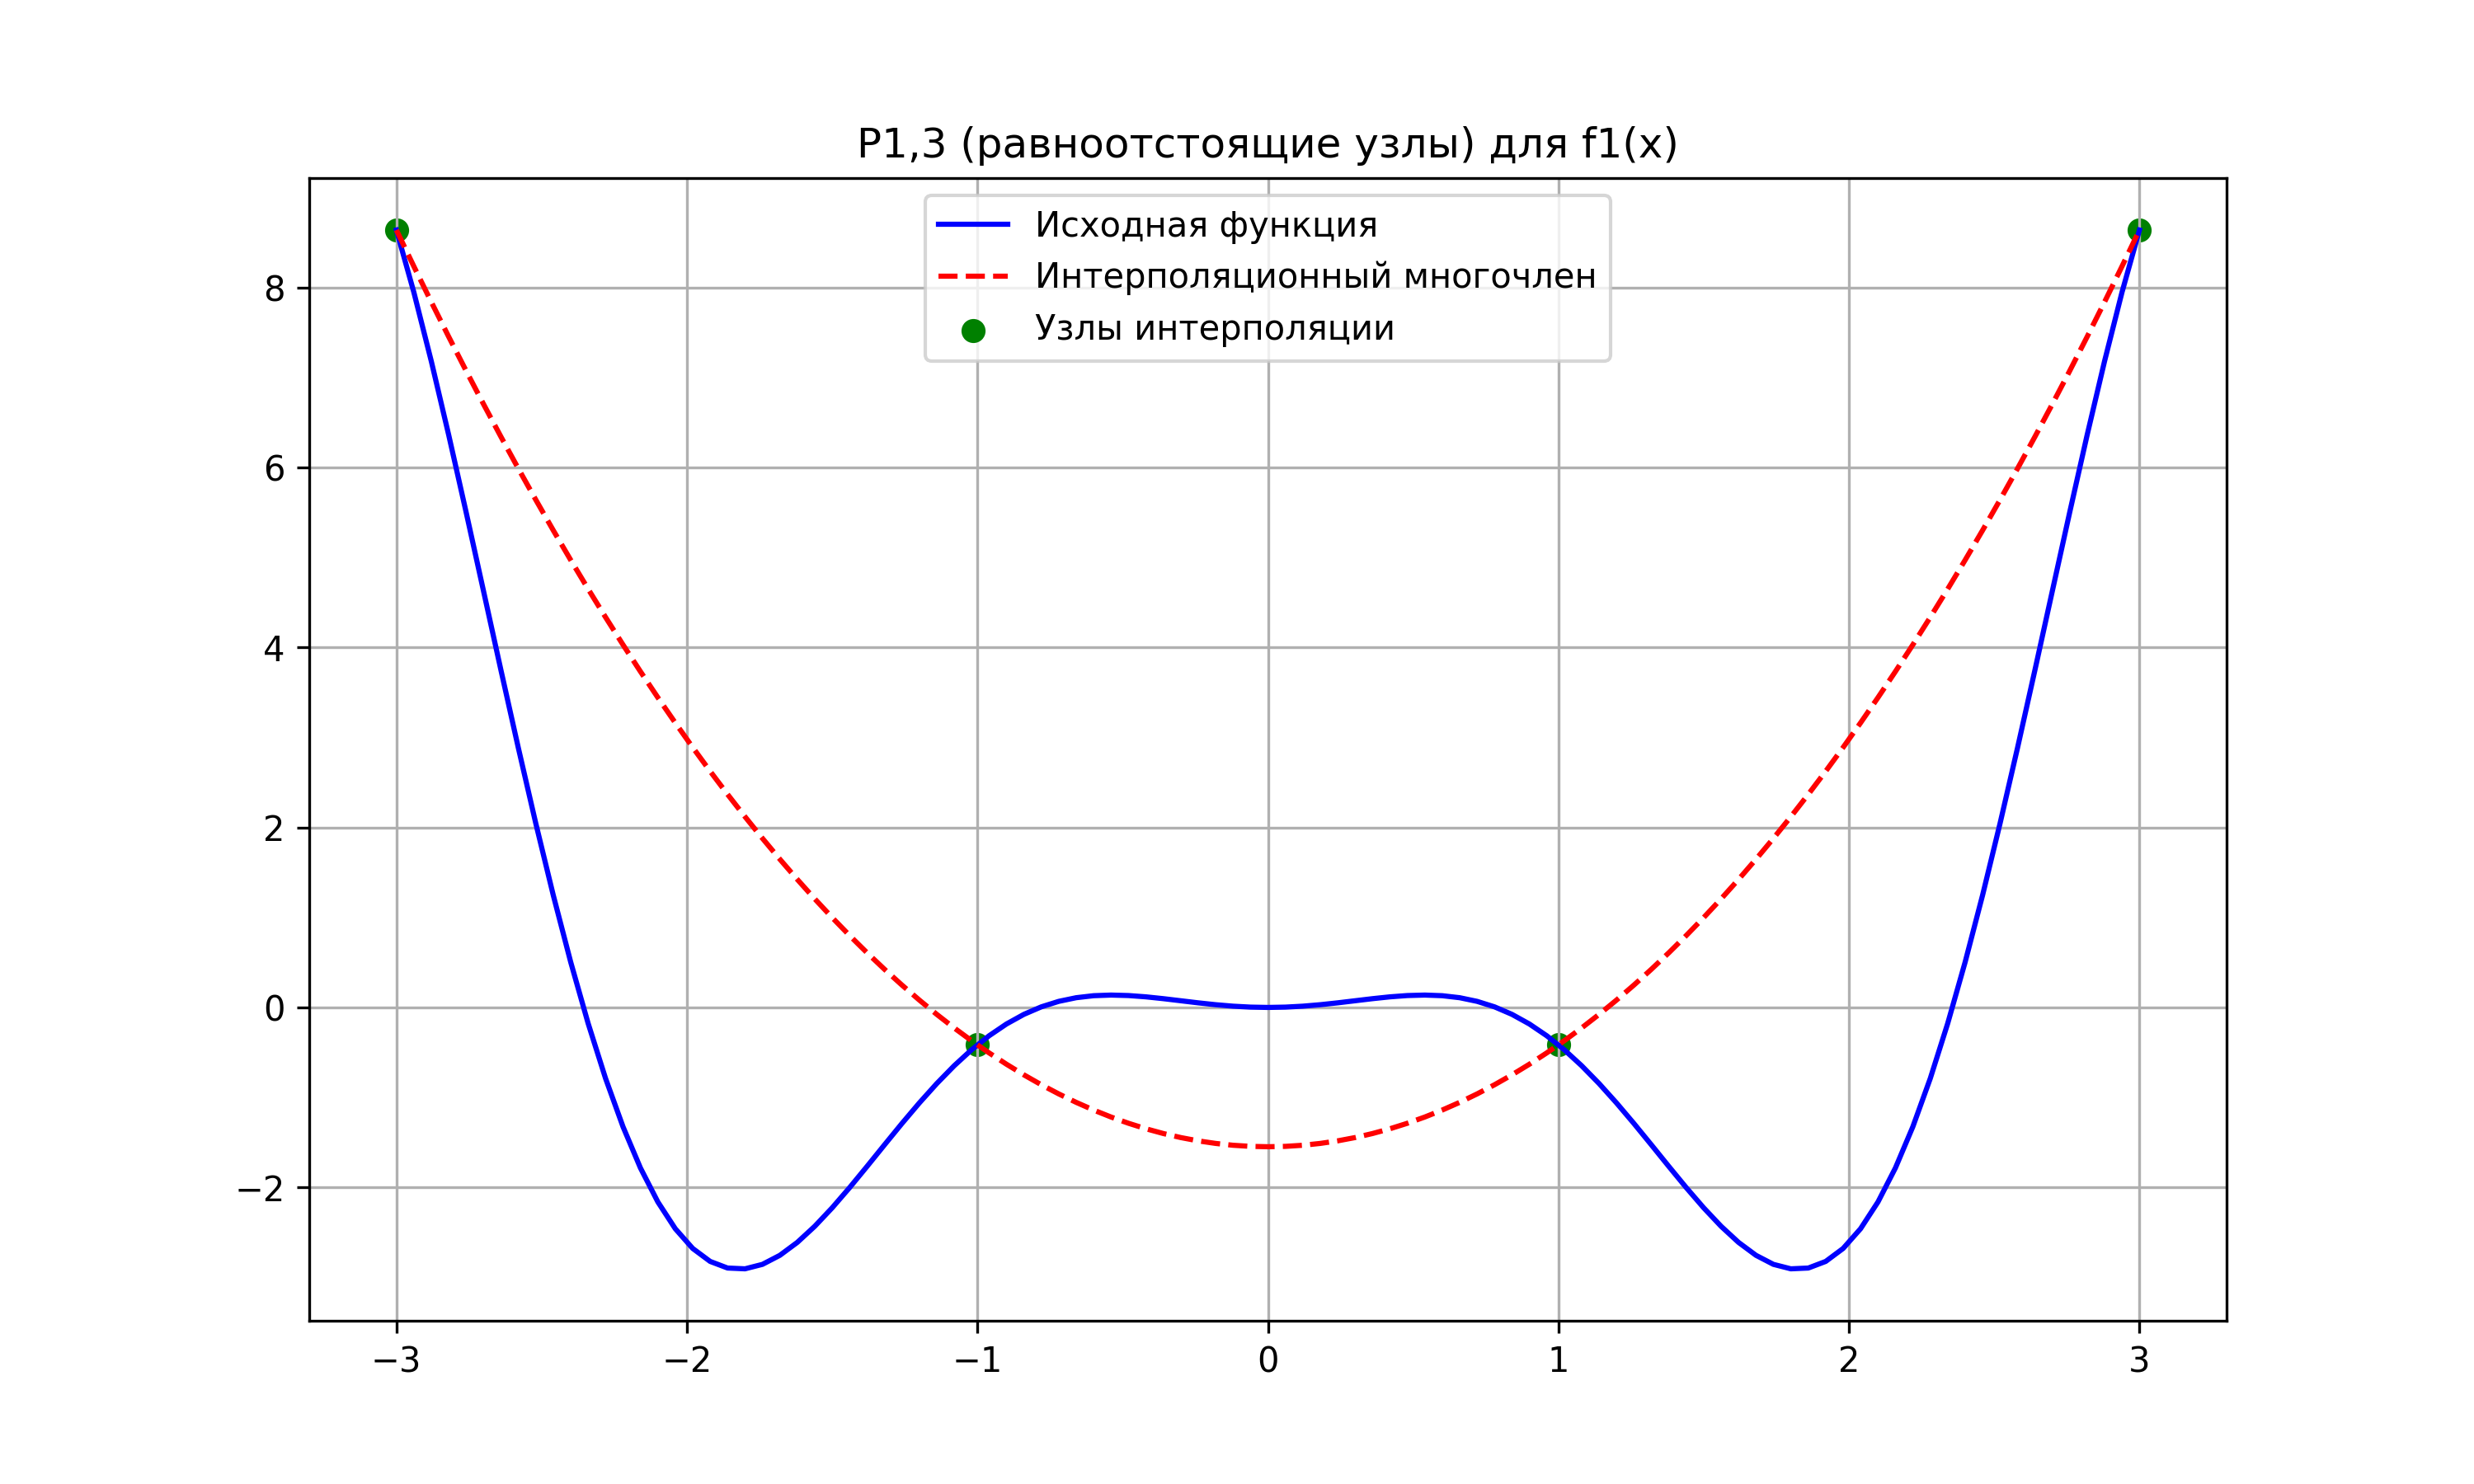
\includegraphics[width=0.8\textwidth]{P1_3.png}
    \caption{Интерполяция $f_1(x)$ по равноотстоящим узлам, $n=3$}
\end{figure}

\begin{figure}[H]
    \centering
    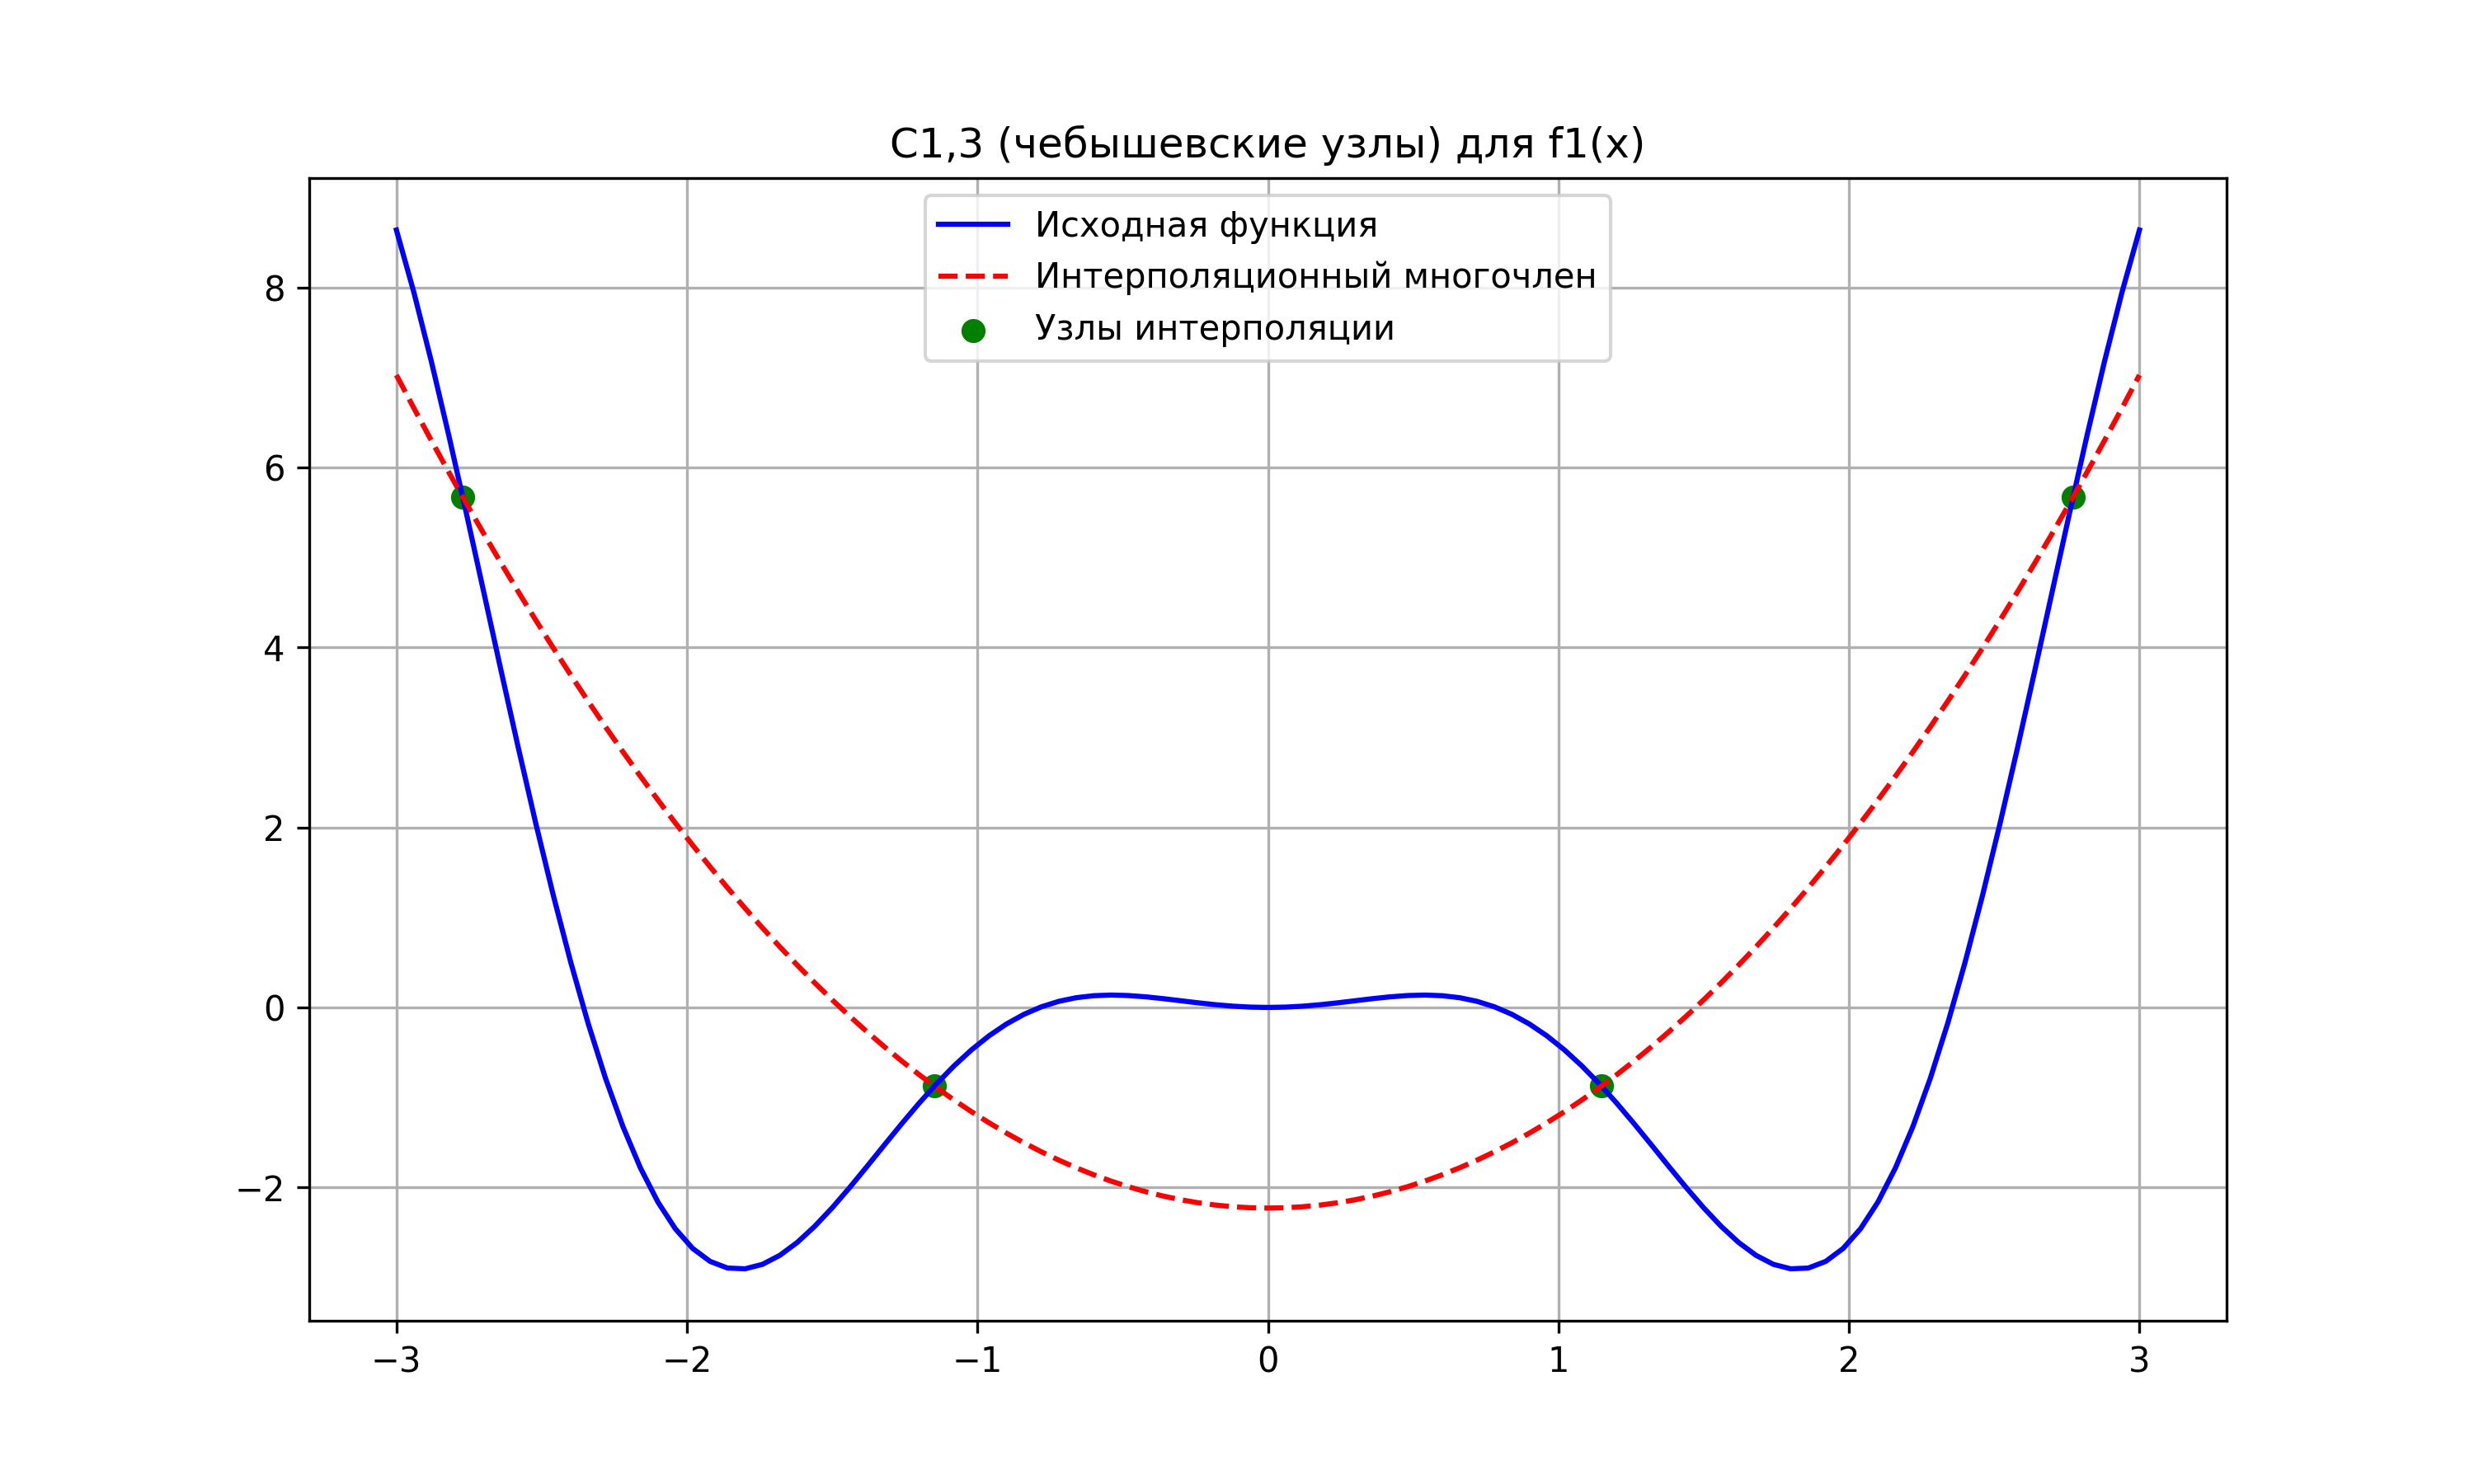
\includegraphics[width=0.8\textwidth]{C1_3.png}
    \caption{Интерполяция $f_1(x)$ по чебышёвским узлам, $n=3$}
\end{figure}

\begin{figure}[H]
    \centering
    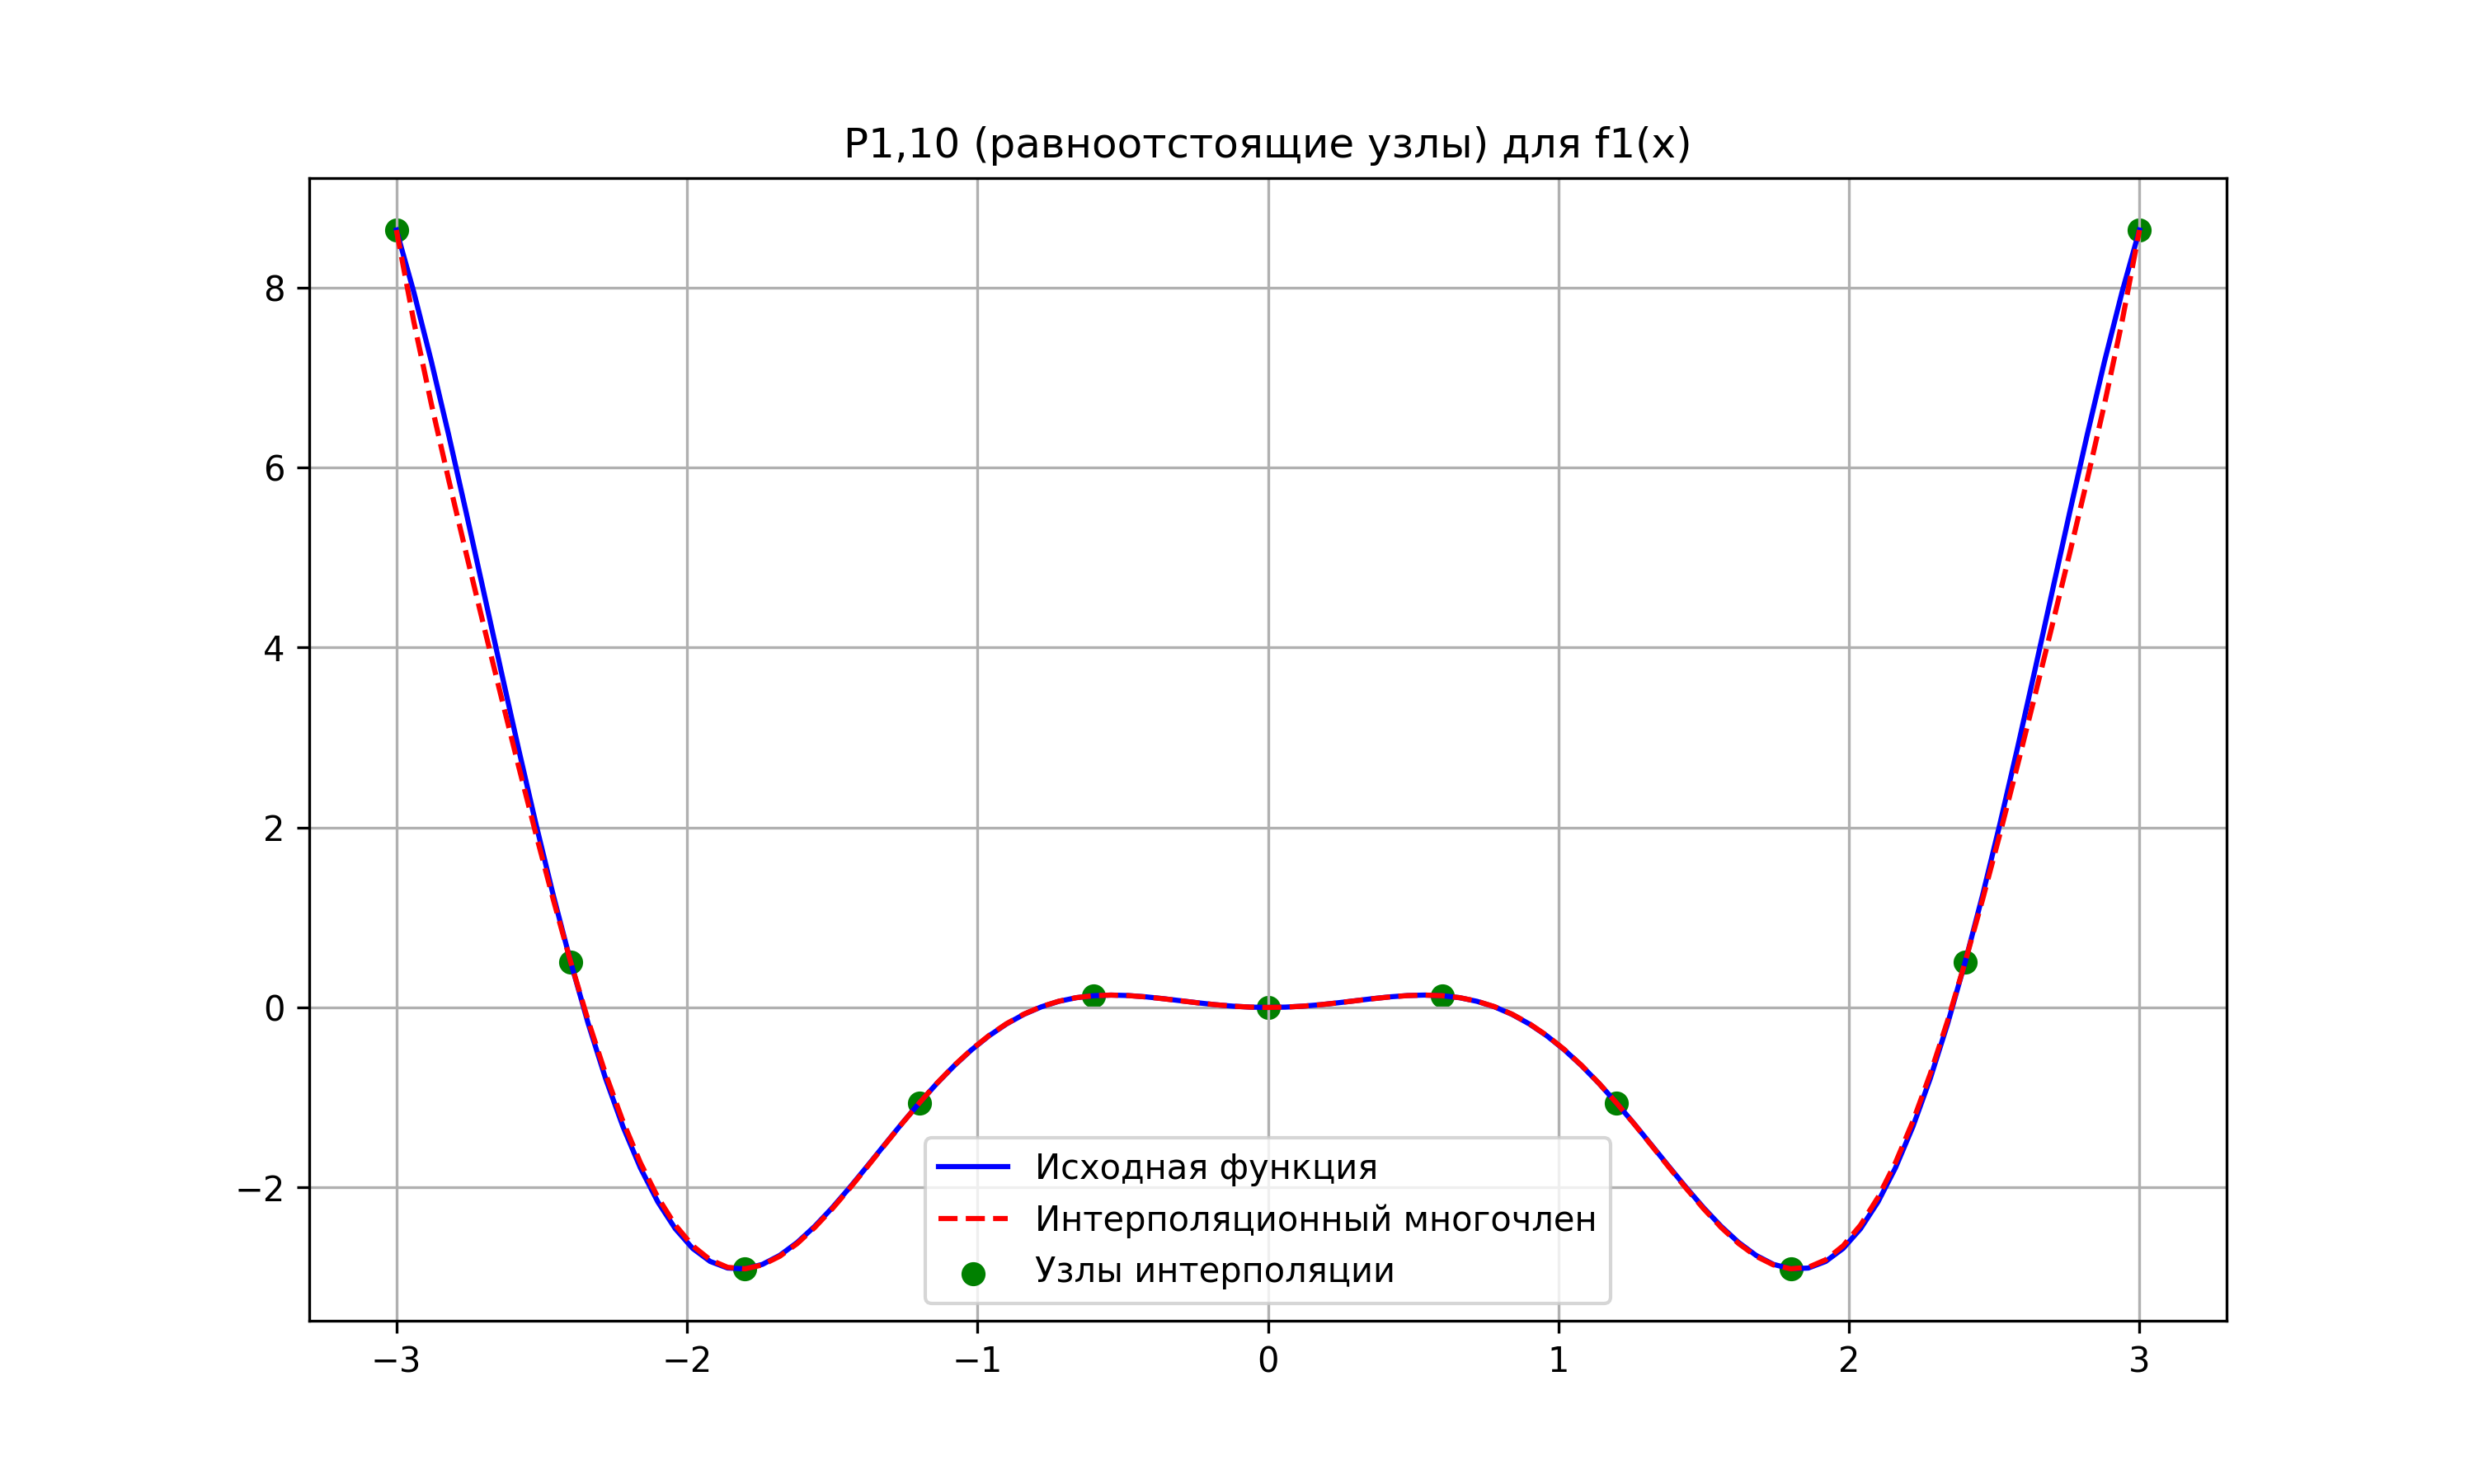
\includegraphics[width=0.8\textwidth]{P1_10.png}
    \caption{Интерполяция $f_1(x)$ по равноотстоящим узлам, $n=10$}
\end{figure}

\begin{figure}[H]
    \centering
    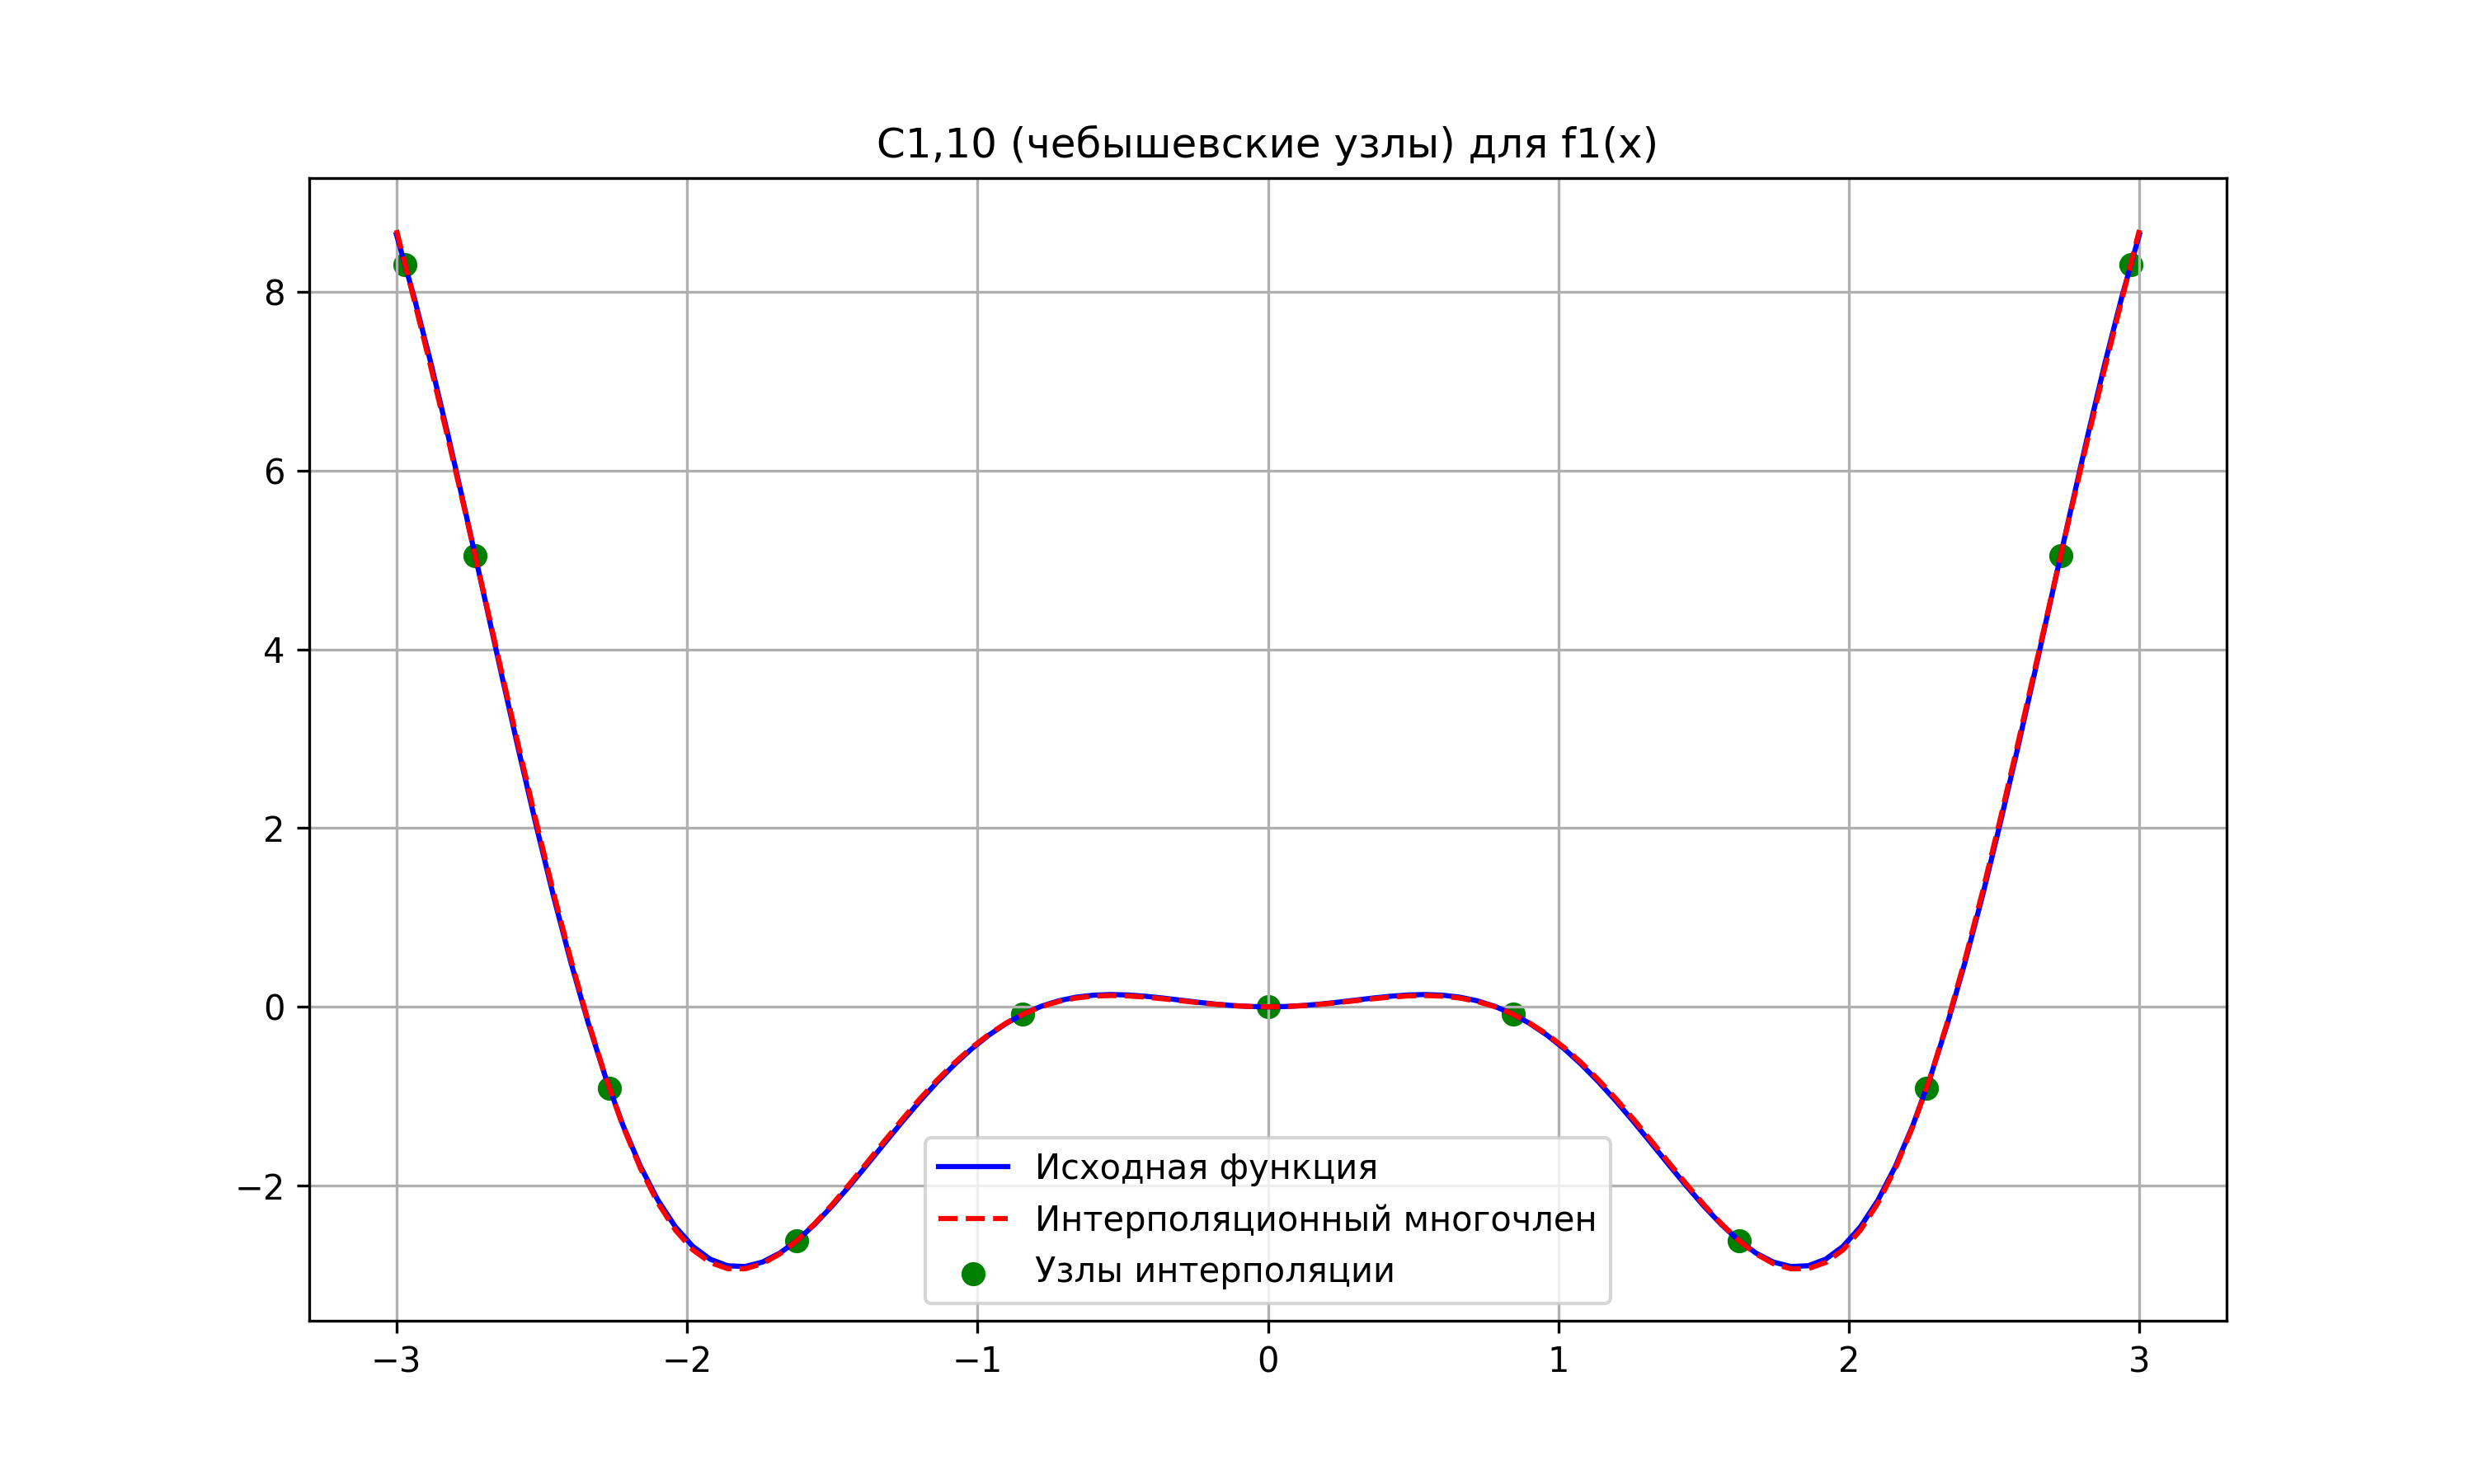
\includegraphics[width=0.8\textwidth]{C1_10.png}
    \caption{Интерполяция $f_1(x)$ по чебышёвским узлам, $n=10$}
\end{figure}

\begin{figure}[H]
    \centering
    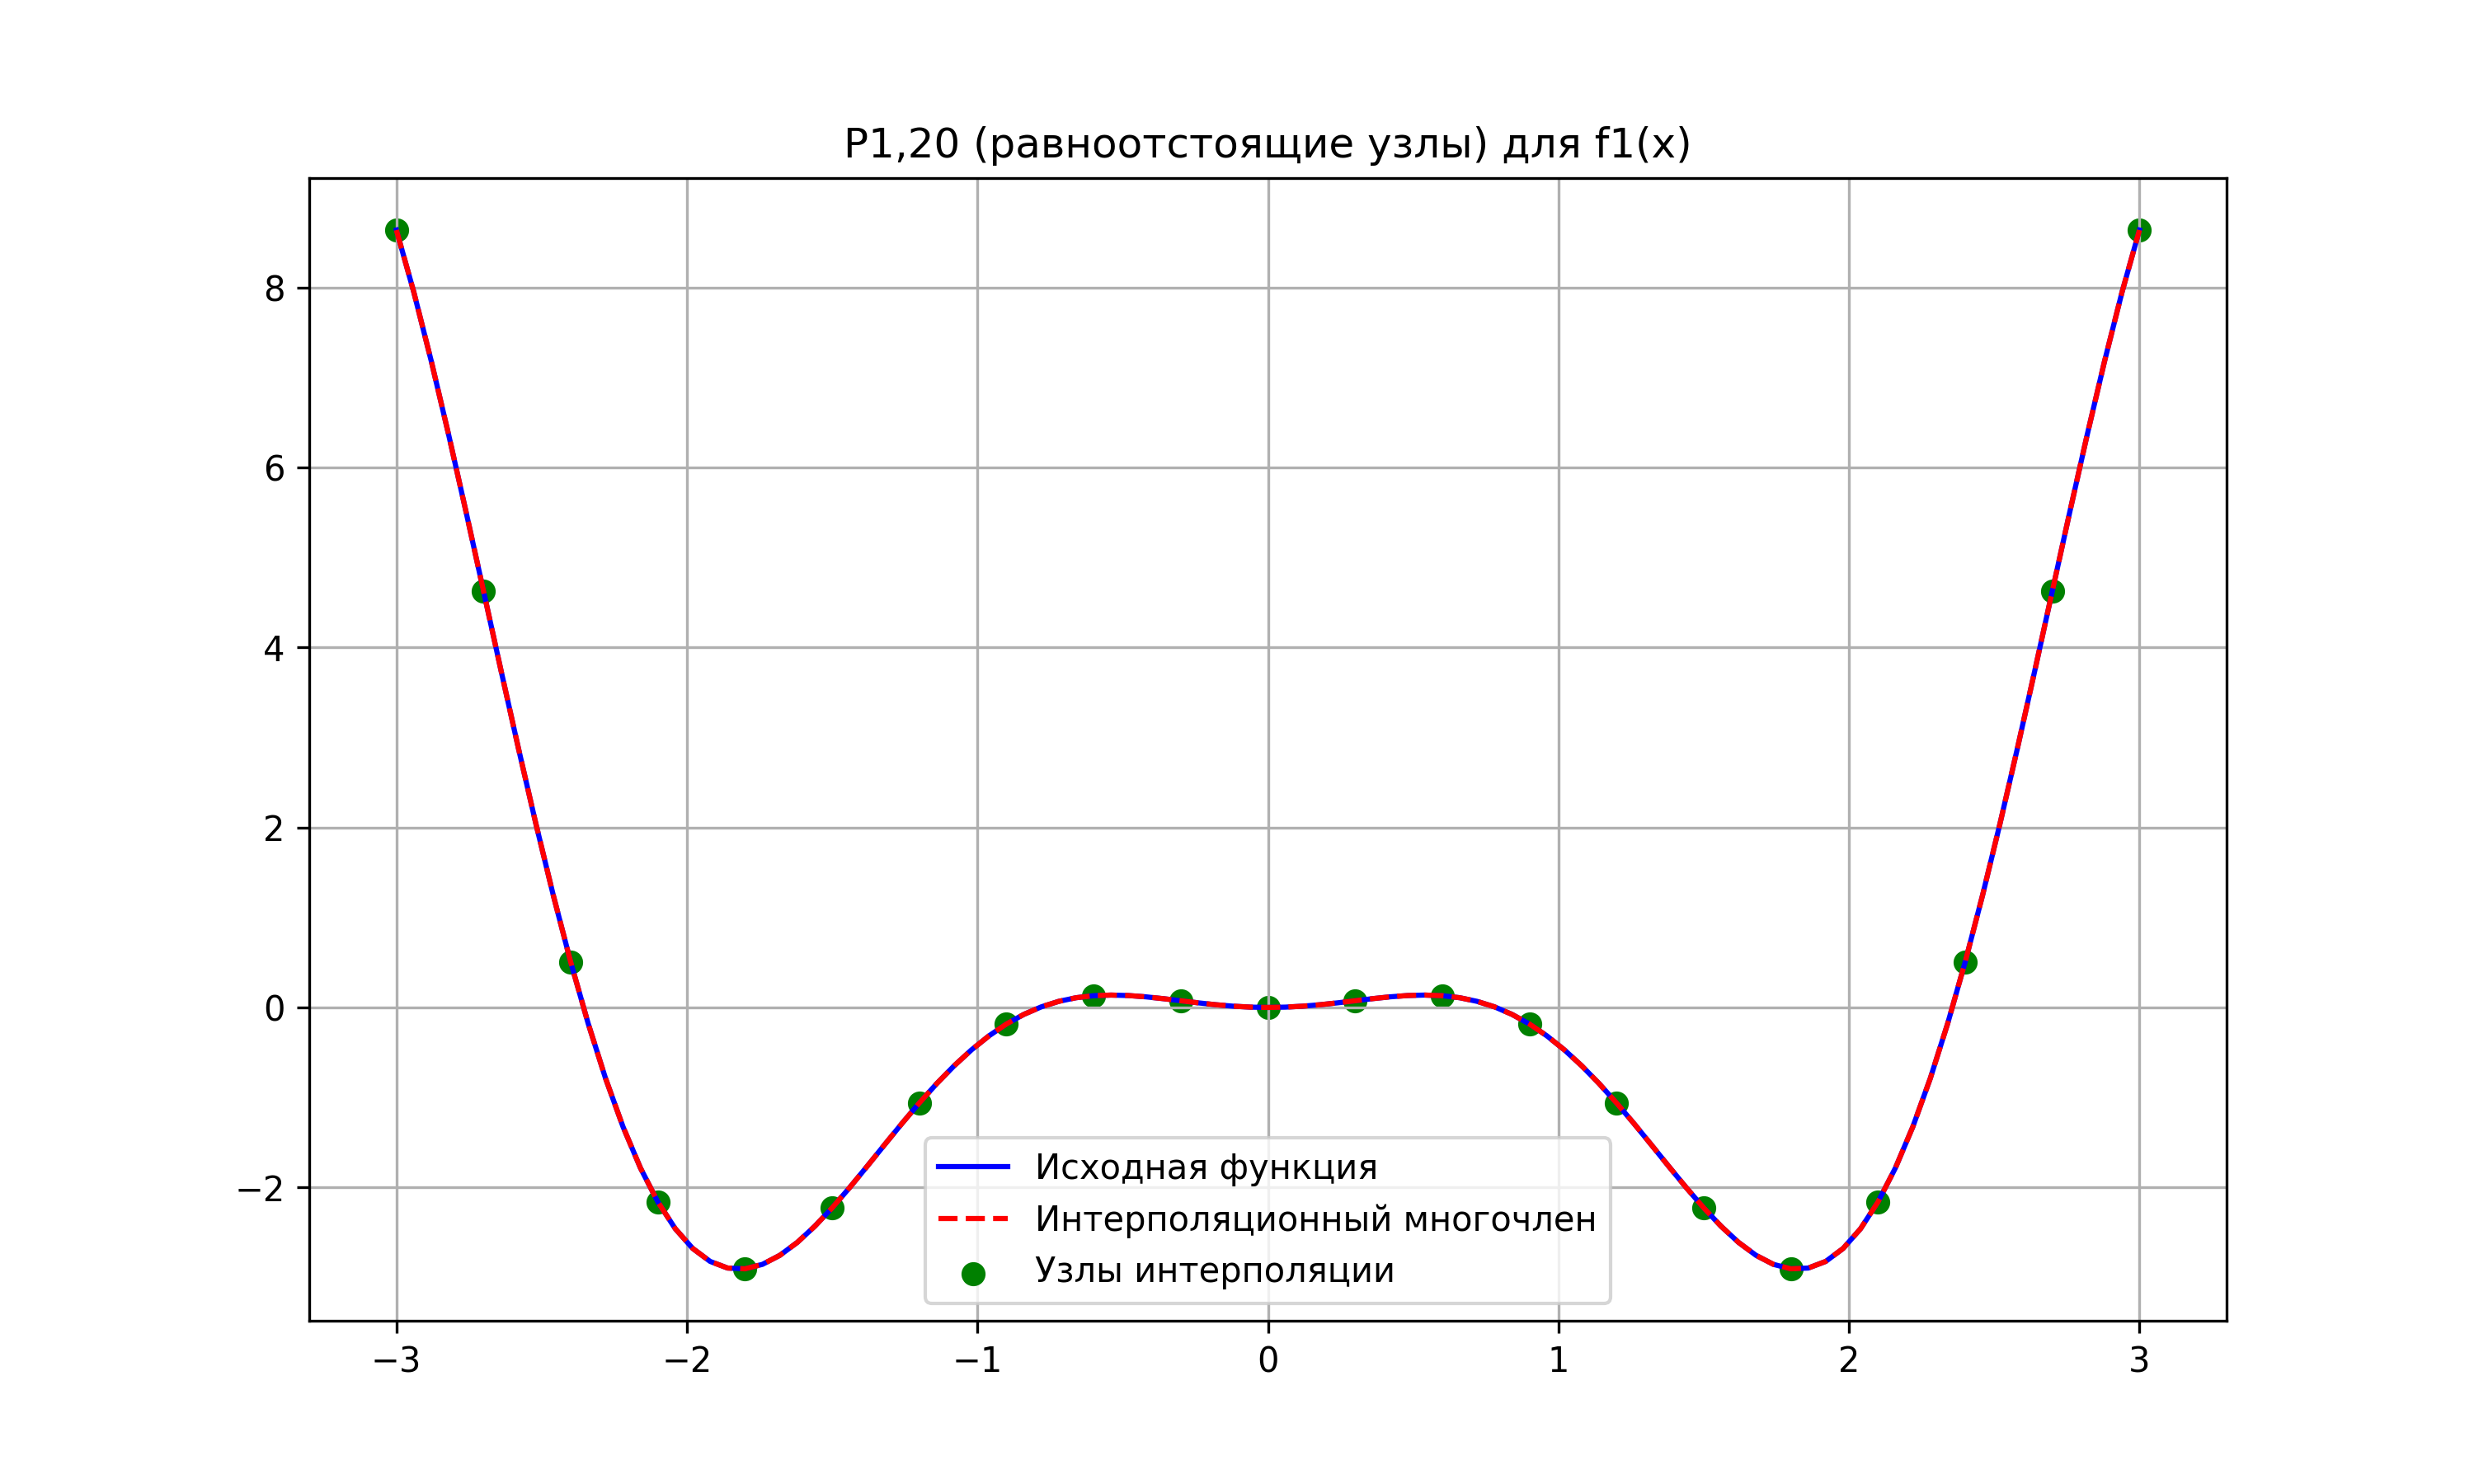
\includegraphics[width=0.8\textwidth]{P1_20.png}
    \caption{Интерполяция $f_1(x)$ по равноотстоящим узлам, $n=20$}
\end{figure}

\begin{figure}[H]
    \centering
    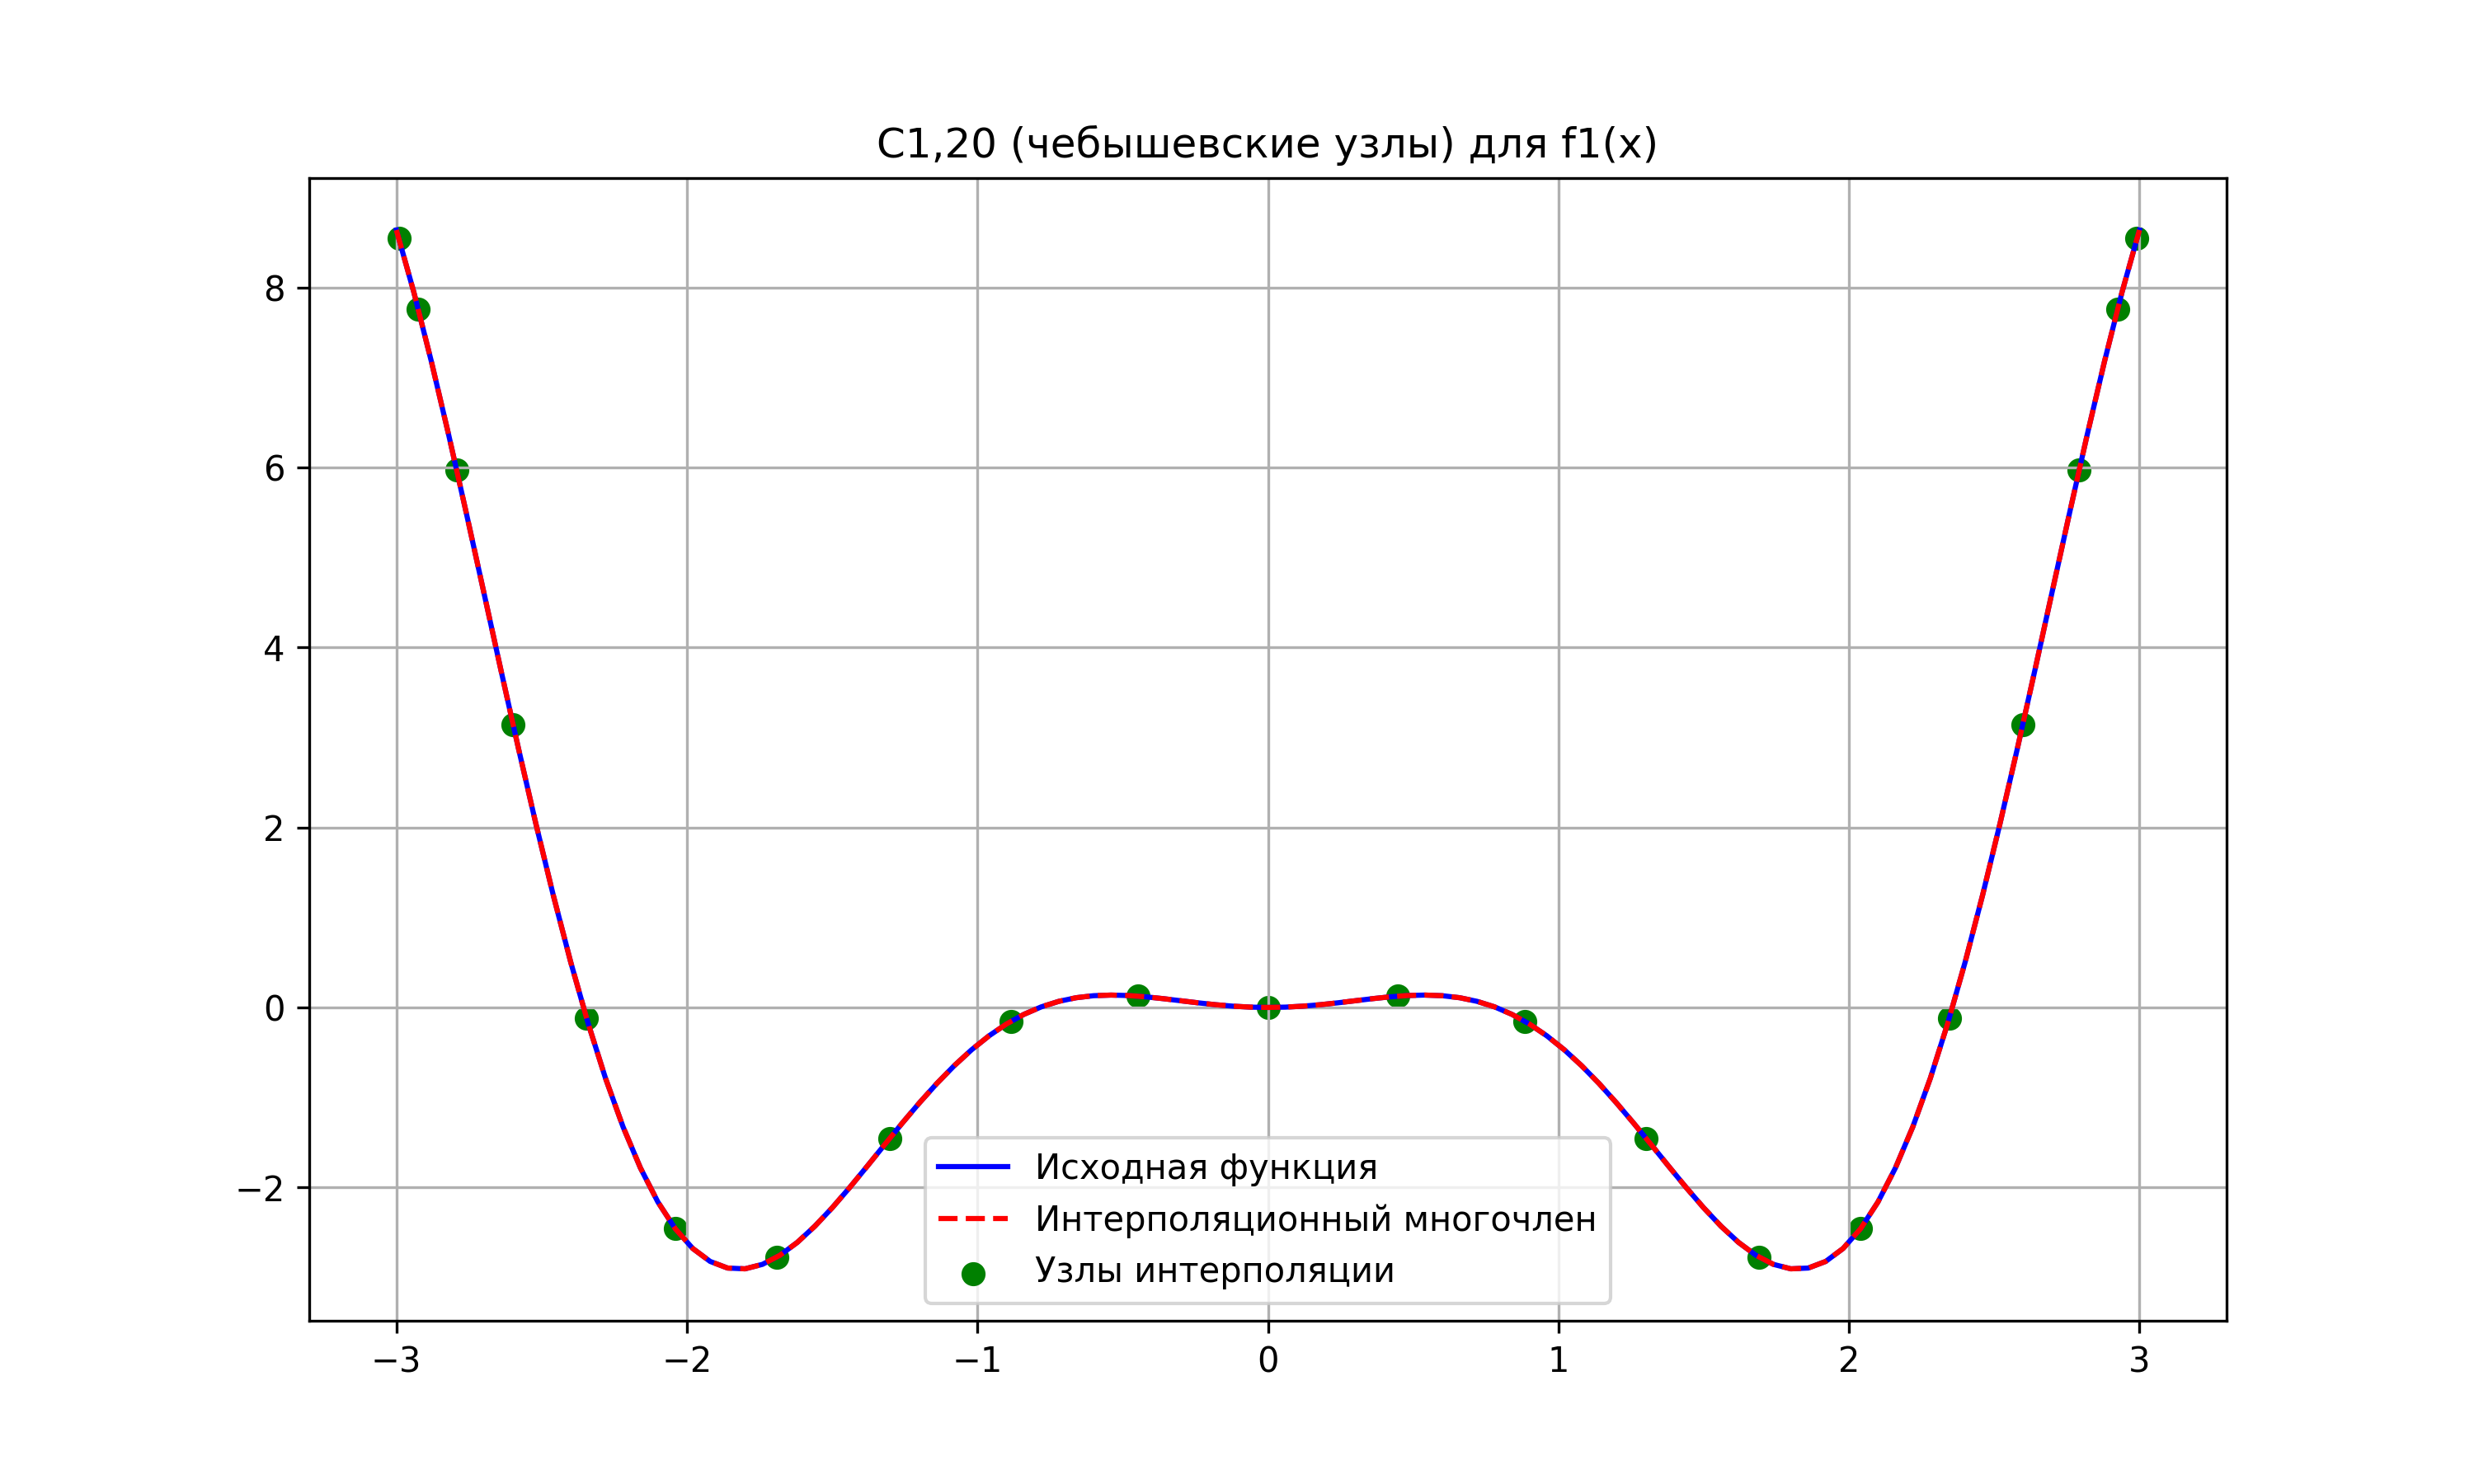
\includegraphics[width=0.8\textwidth]{C1_20.png}
    \caption{Интерполяция $f_1(x)$ по чебышёвским узлам, $n=20$}
\end{figure}

\subsection{Погрешности интерполяции}

\begin{table}[H]
    \centering
    \begin{tabular}{|c|c|c|}
        \hline
        $n$ & $\max\limits_{i=0,100} |P_{1,n}(x_i) - f_1(x_i)|$ & $\max\limits_{i=0,100} |C_{1,n}(x_i) - f_1(x_i)|$ \\
        \hline
        5 & 1.865255e+00 & 1.354988e+00 \\
        \hline
        10 & 4.986315e-01 & 4.898594e-02 \\
        \hline
        15 & 5.873508e-03 & 1.337354e-04 \\
        \hline
        20 & 2.077667e-06 & 7.869950e-09 \\
        \hline
        30 & 4.636203e-11 & 2.667733e-11 \\
        \hline
    \end{tabular}
    \caption{Погрешности интерполяции функции $f_1(x)$}
\end{table}

\section{Результаты интерполяции для функции $f_2(x) = \frac{1}{1 + 5x^2}$}

\subsection{Графики интерполяционных многочленов}

\begin{figure}[H]
    \centering
    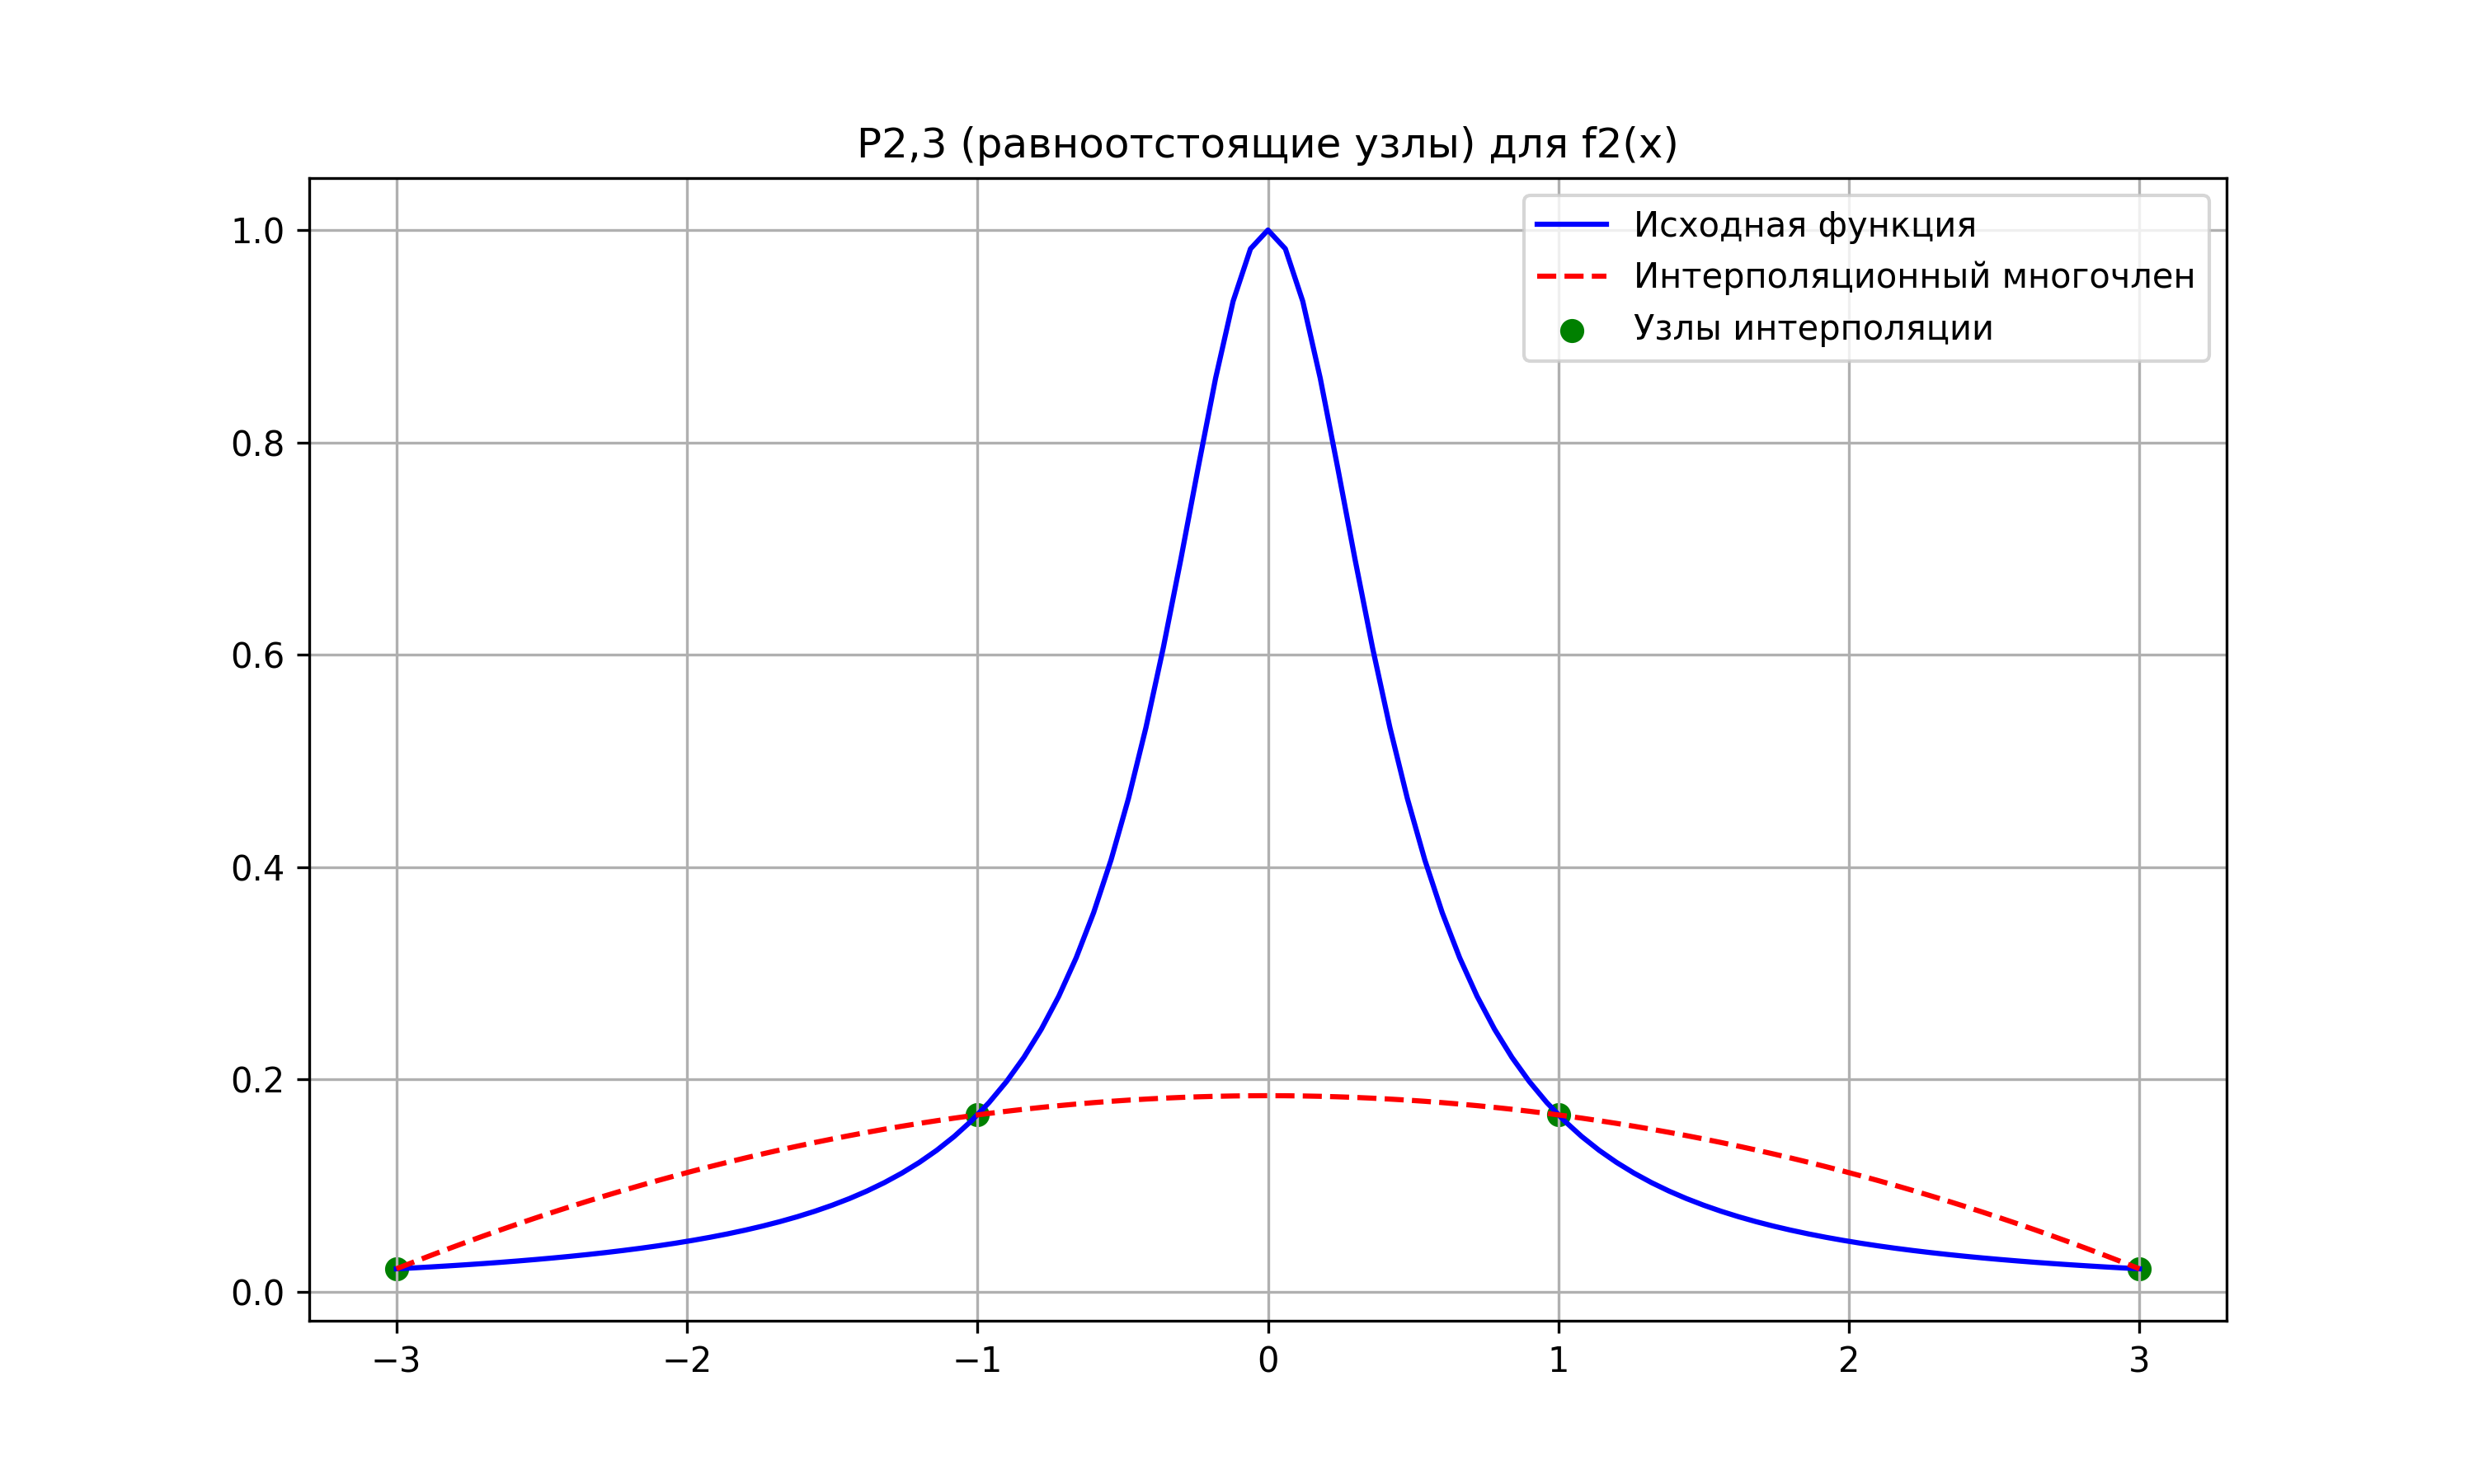
\includegraphics[width=0.8\textwidth]{P2_3.png}
    \caption{Интерполяция $f_2(x)$ по равноотстоящим узлам, $n=3$}
\end{figure}

\begin{figure}[H]
    \centering
    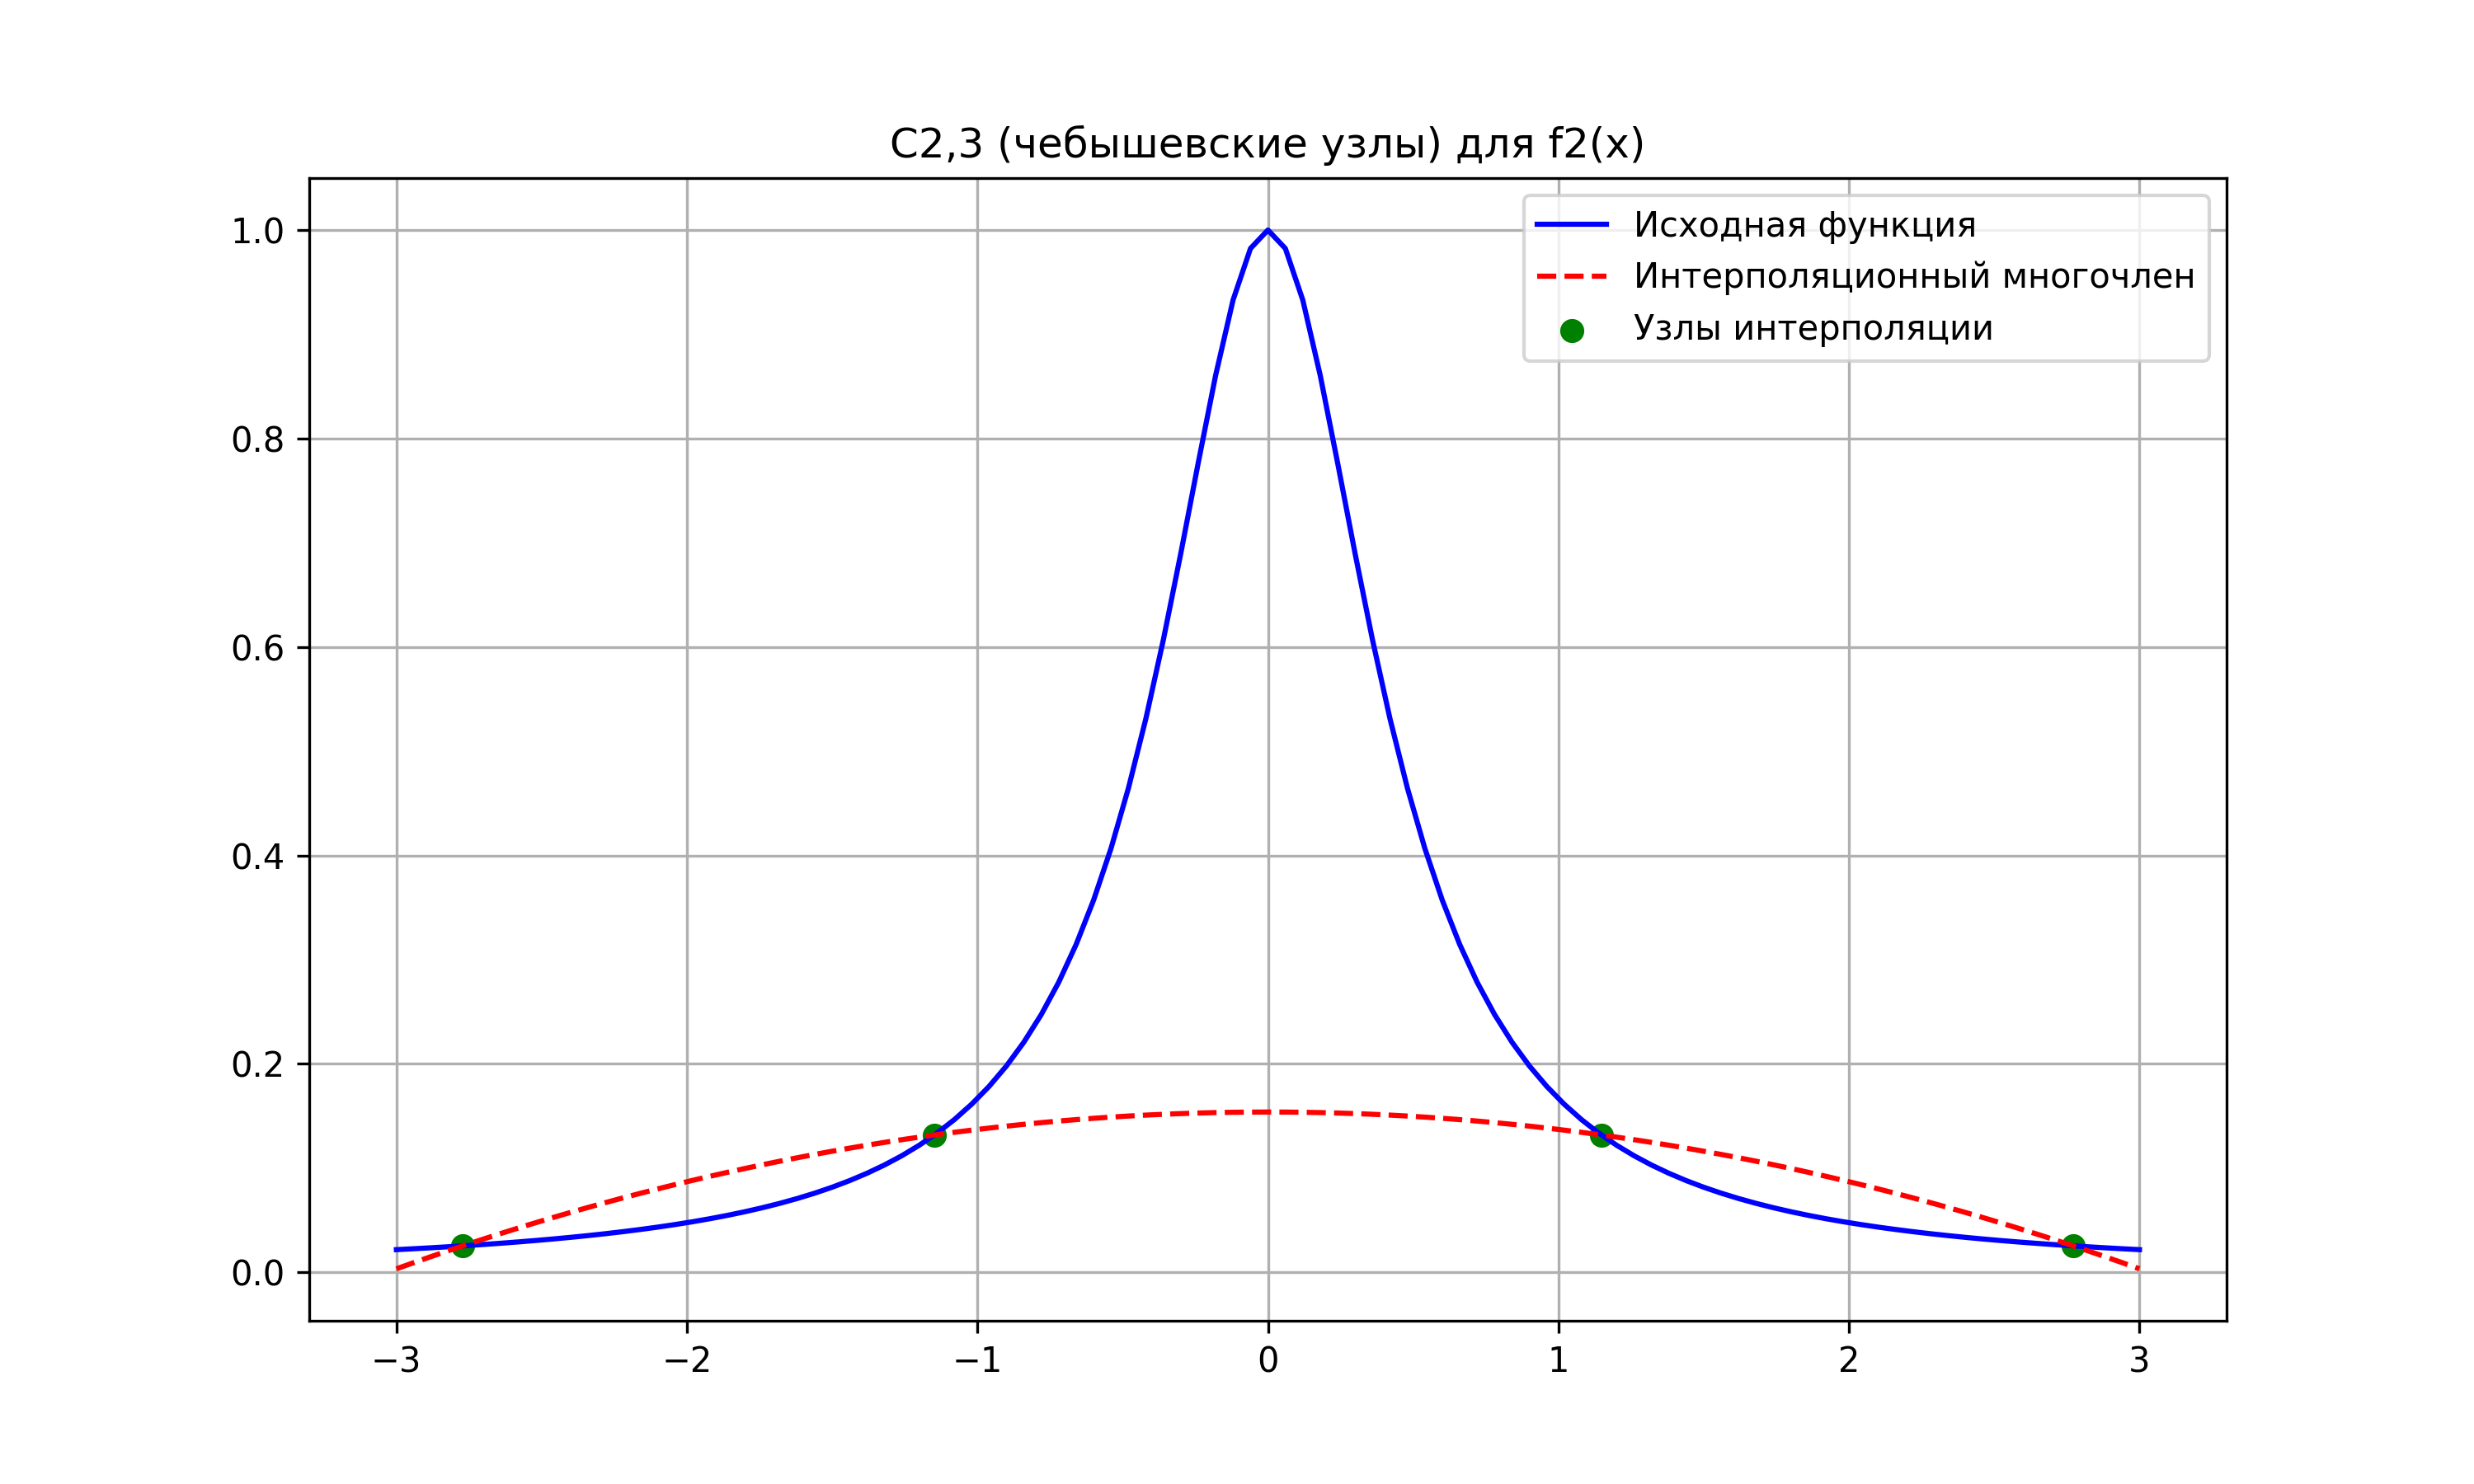
\includegraphics[width=0.8\textwidth]{C2_3.png}
    \caption{Интерполяция $f_2(x)$ по чебышёвским узлам, $n=3$}
\end{figure}

\begin{figure}[H]
    \centering
    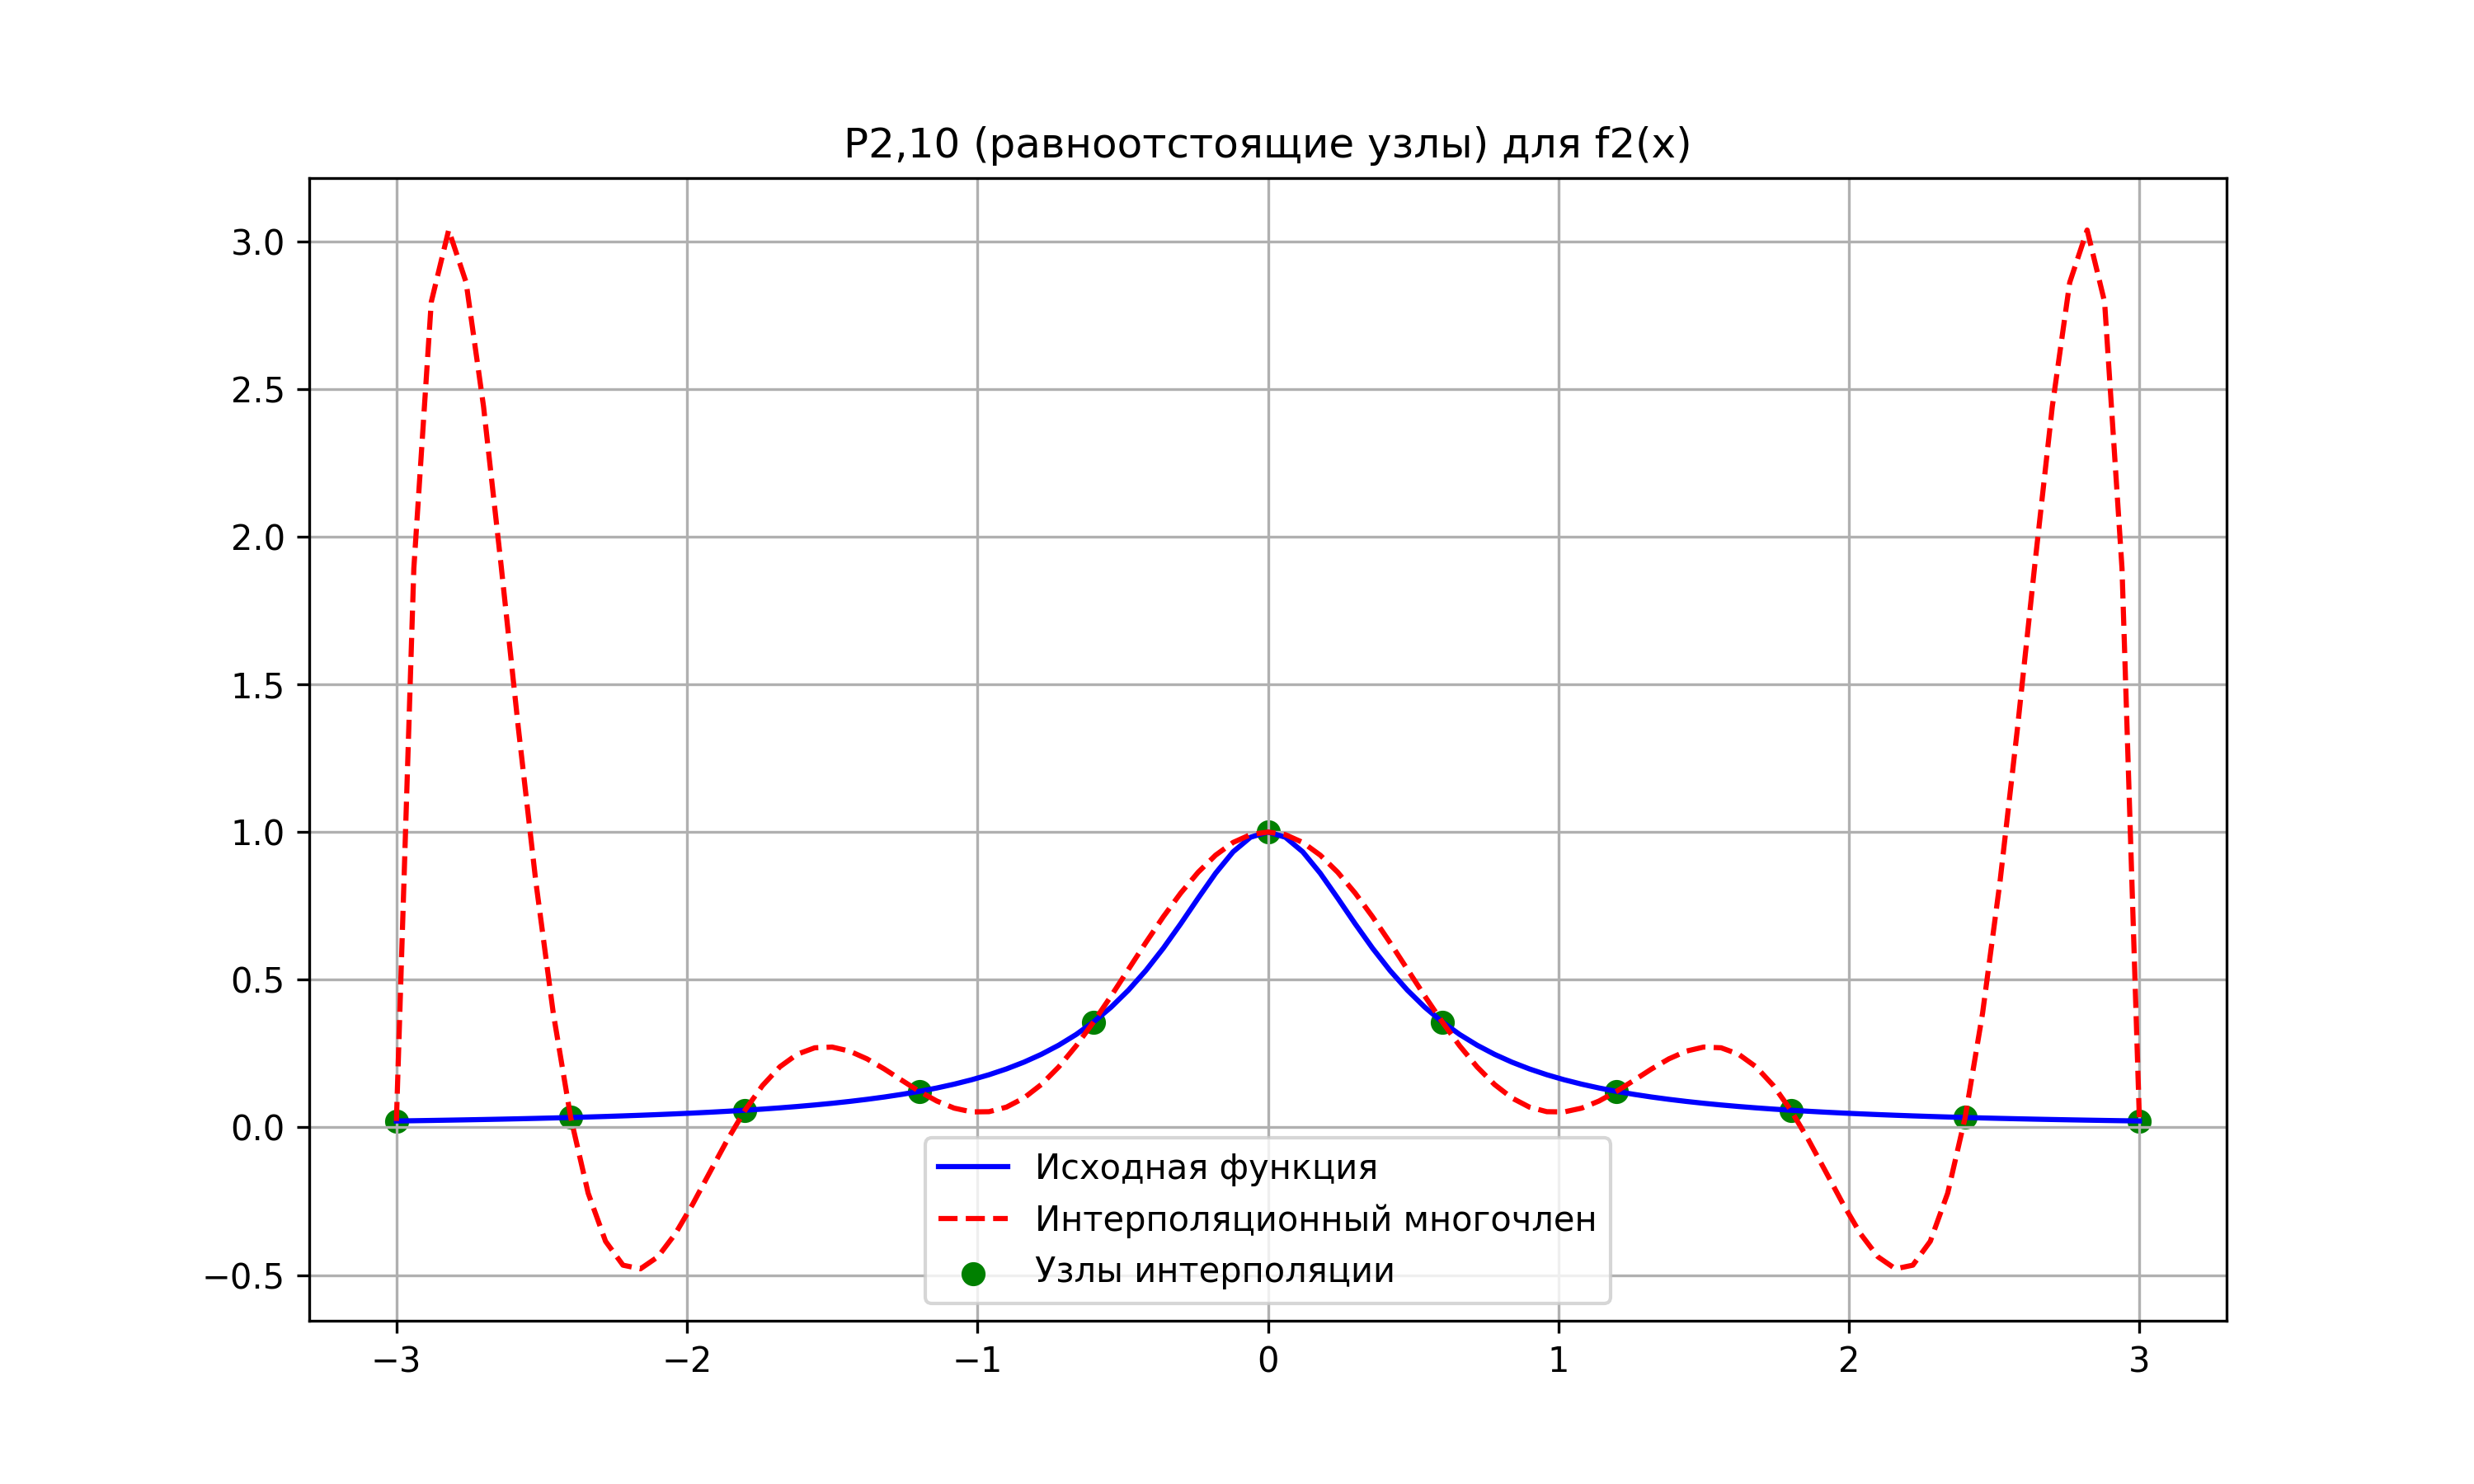
\includegraphics[width=0.8\textwidth]{P2_10.png}
    \caption{Интерполяция $f_2(x)$ по равноотстоящим узлам, $n=10$}
\end{figure}

\begin{figure}[H]
    \centering
    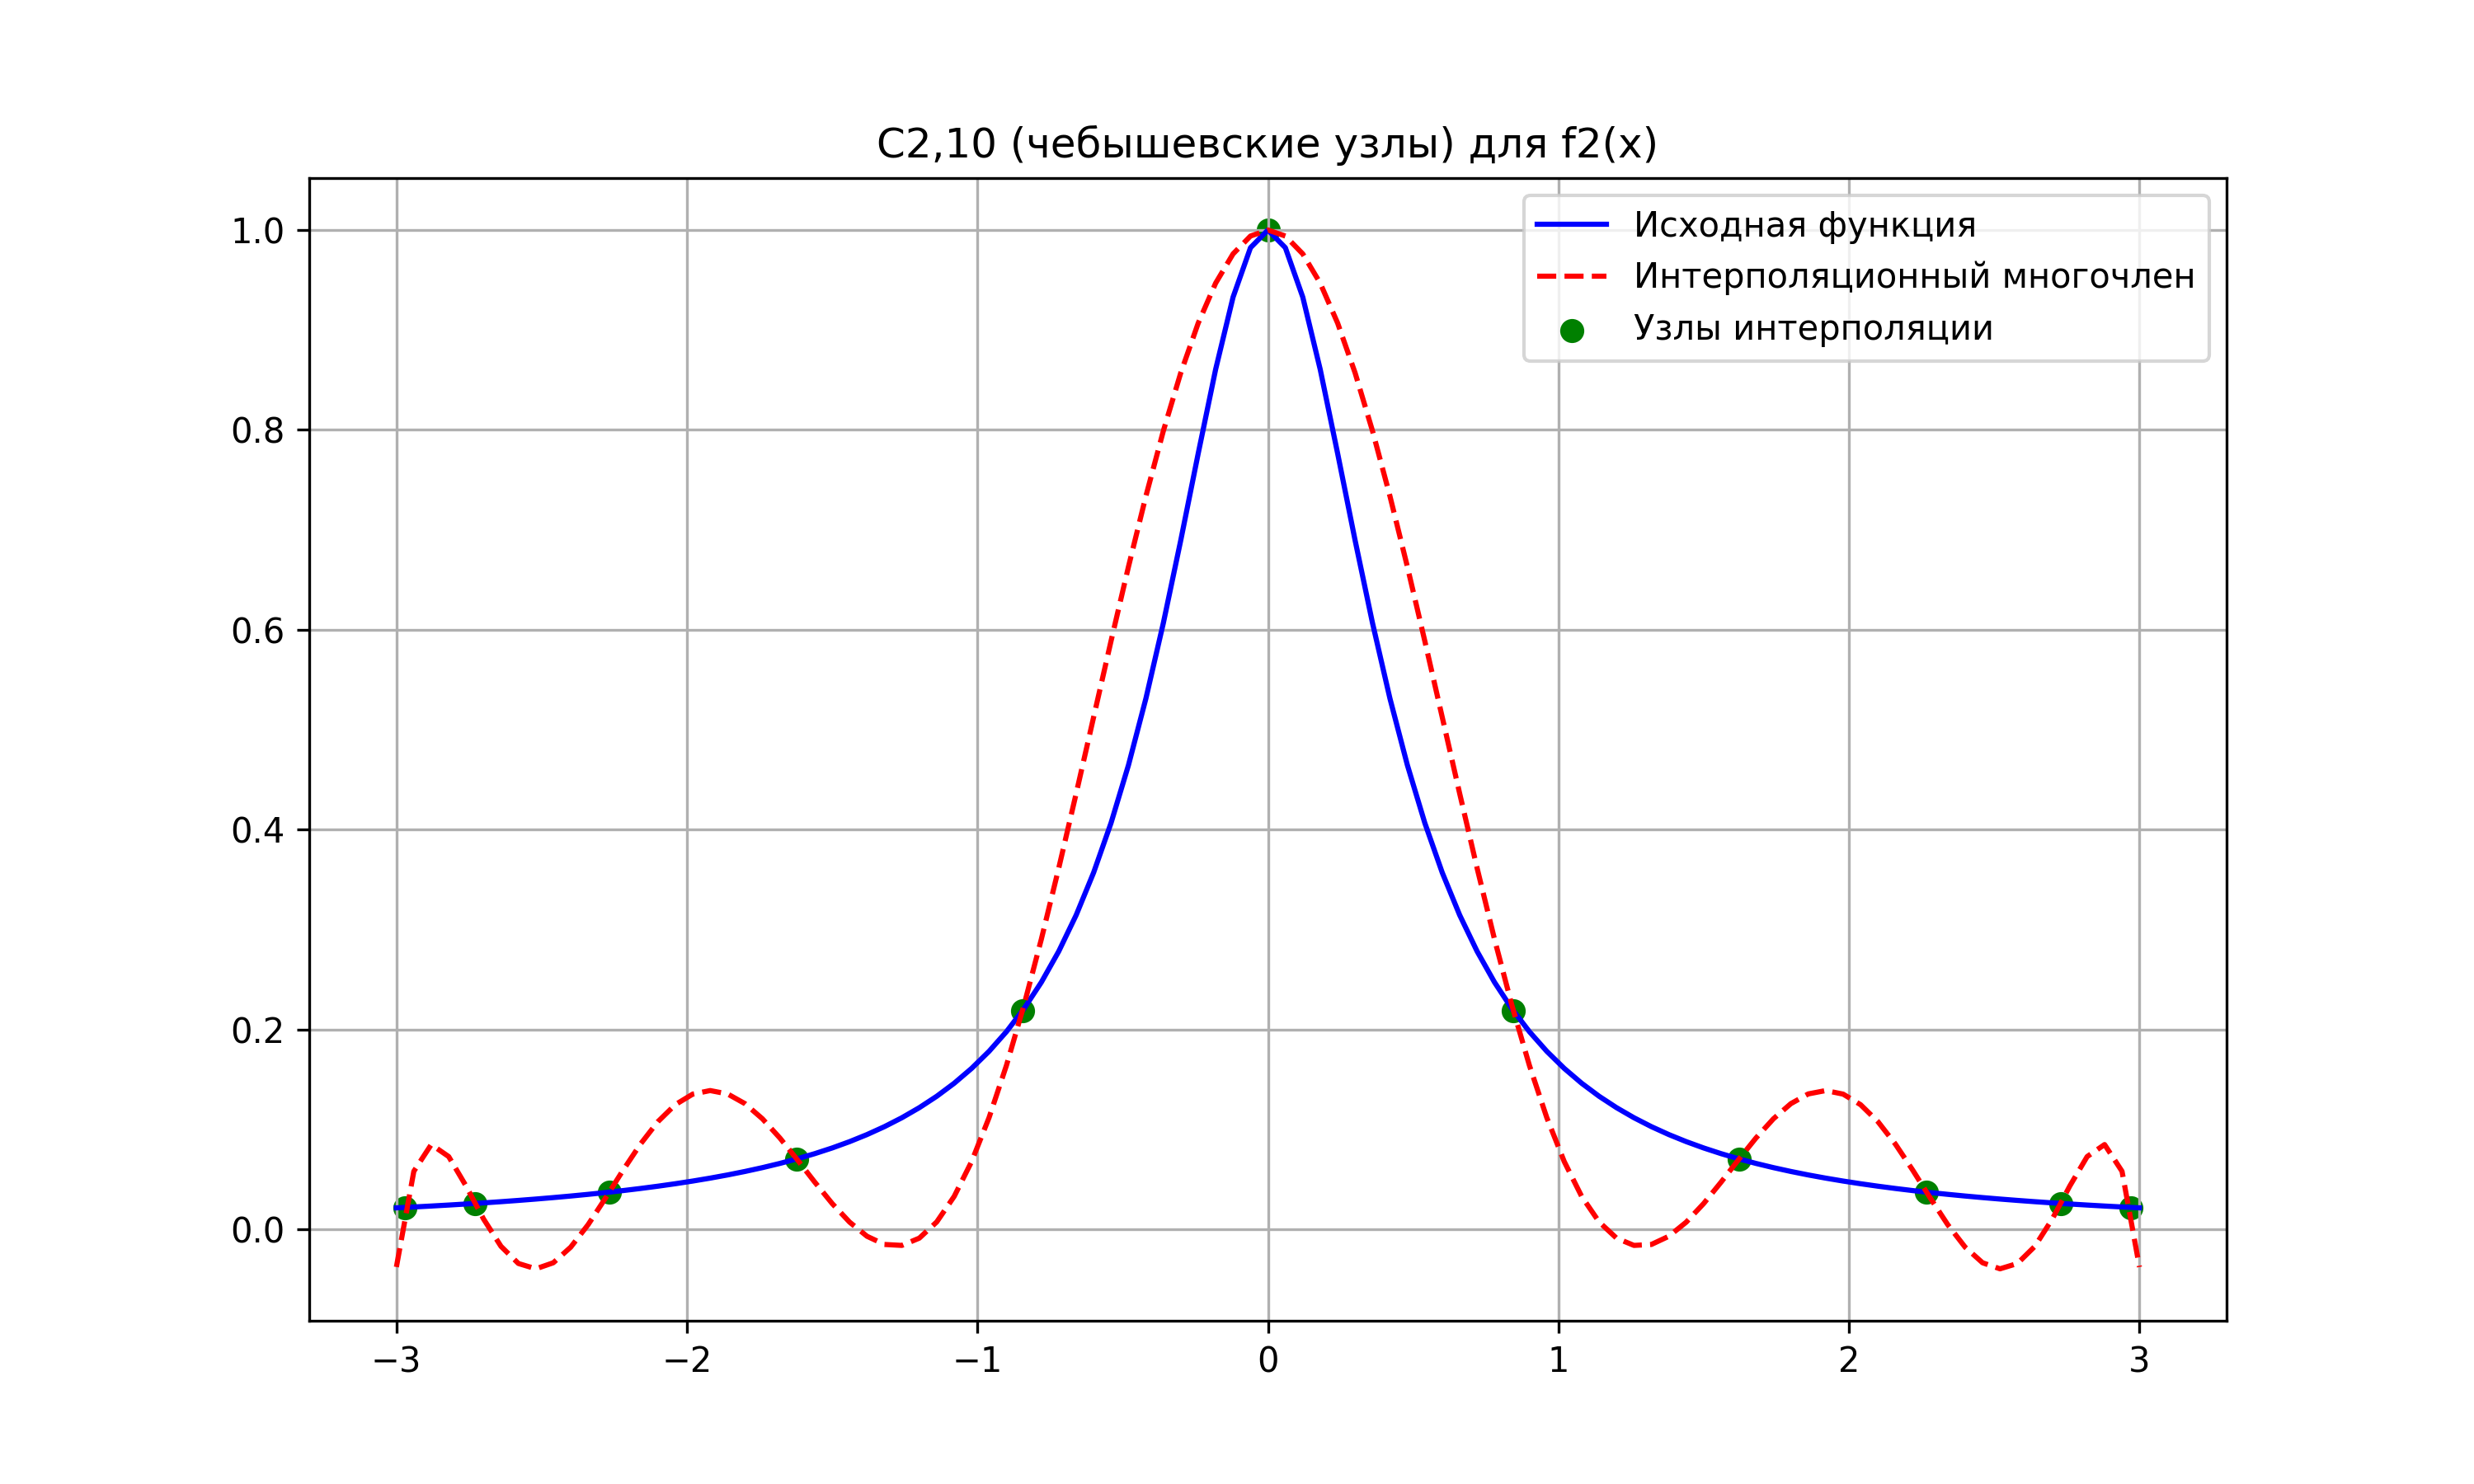
\includegraphics[width=0.8\textwidth]{C2_10.png}
    \caption{Интерполяция $f_2(x)$ по чебышёвским узлам, $n=10$}
\end{figure}

\begin{figure}[H]
    \centering
    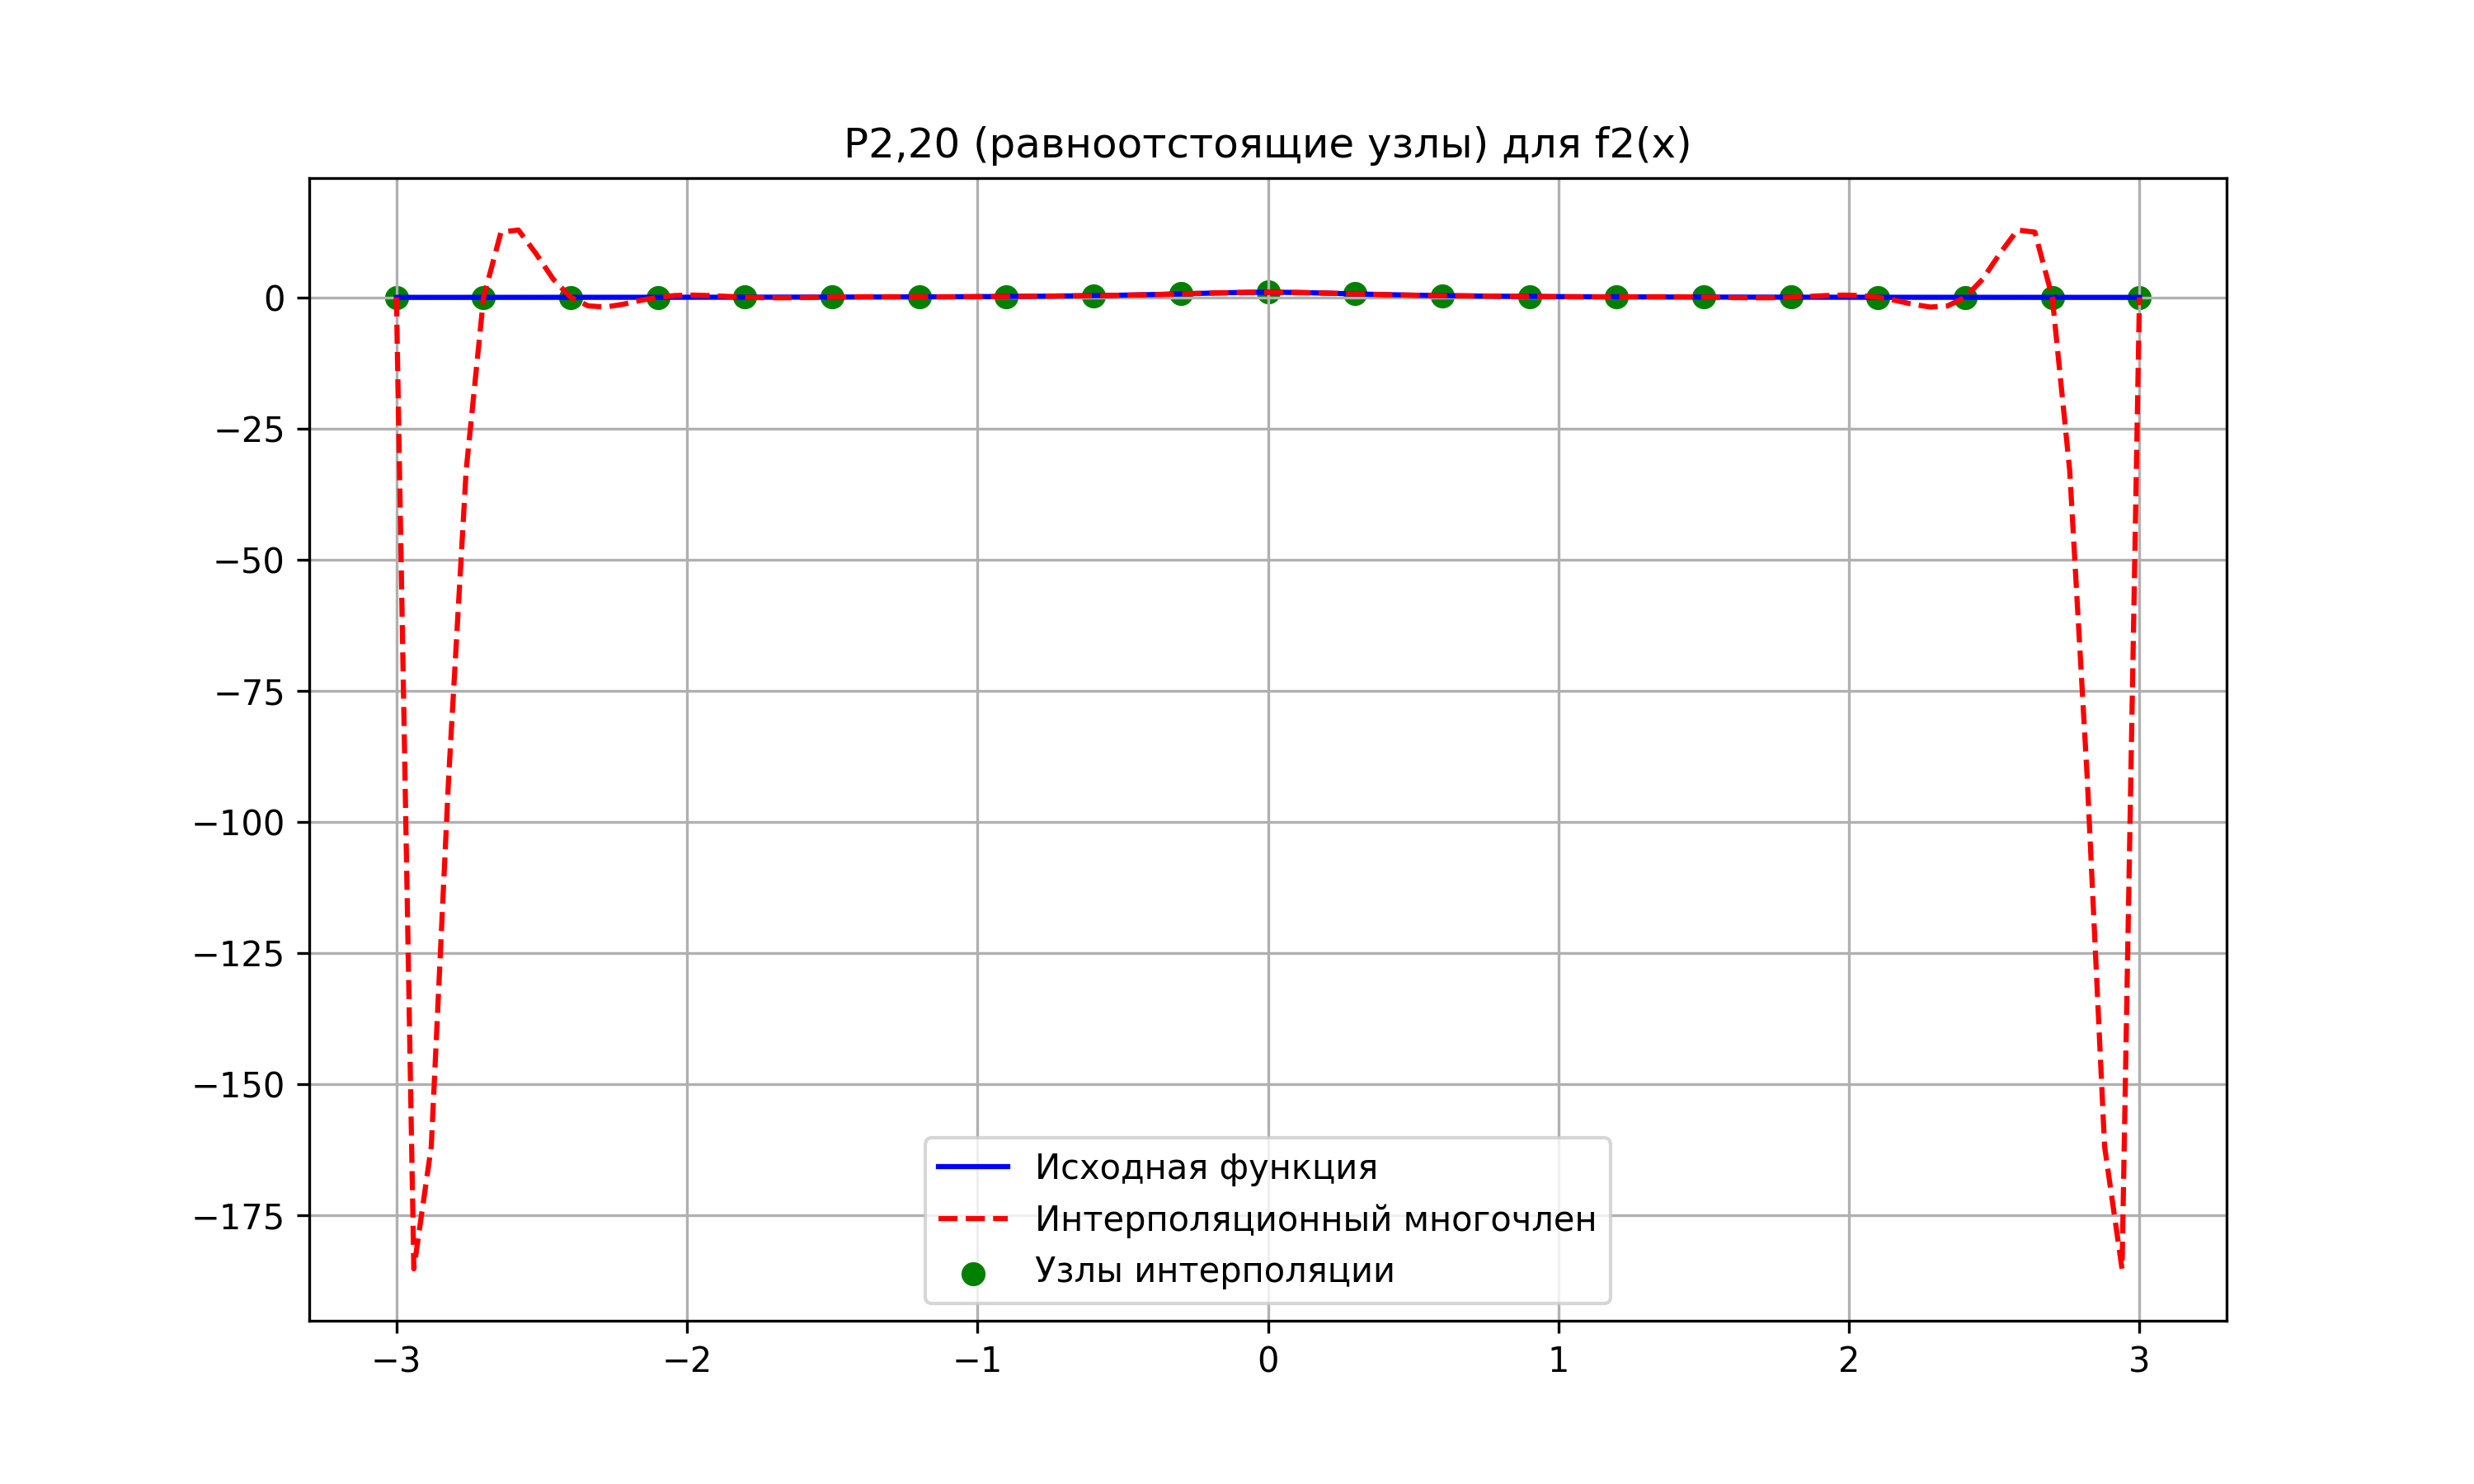
\includegraphics[width=0.8\textwidth]{P2_20.png}
    \caption{Интерполяция $f_2(x)$ по равноотстоящим узлам, $n=20$}
\end{figure}

\begin{figure}[H]
    \centering
    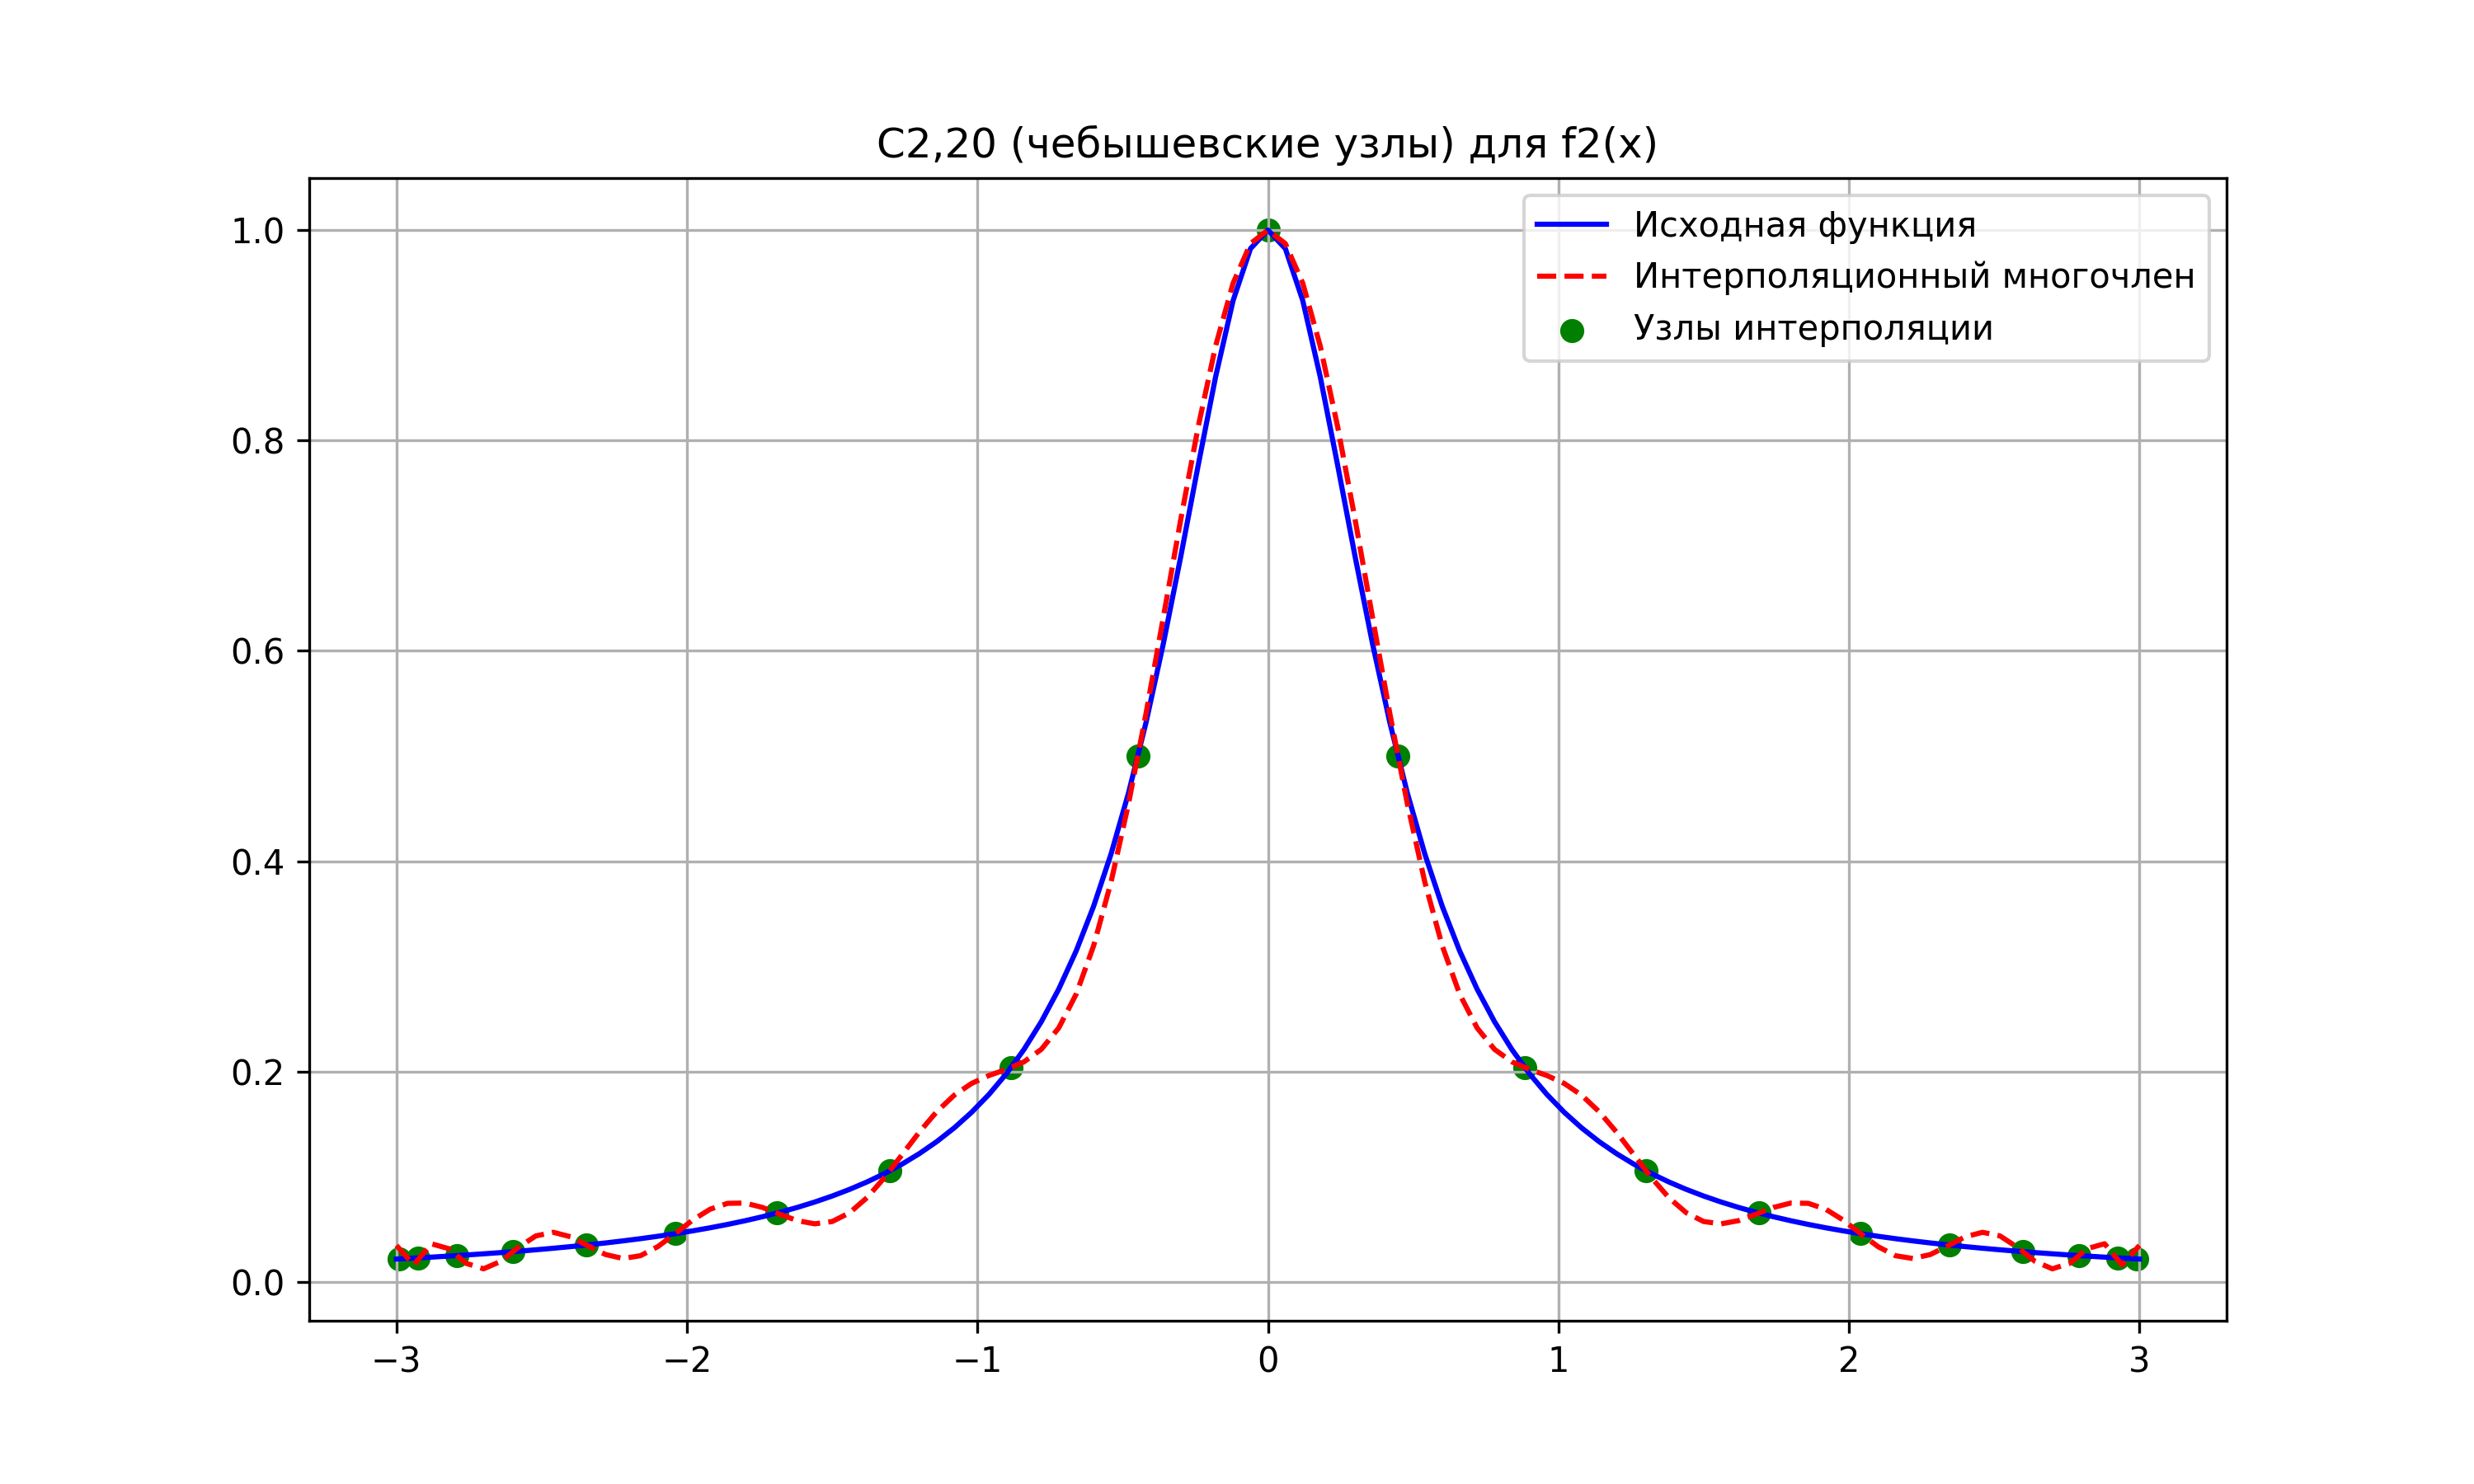
\includegraphics[width=0.8\textwidth]{C2_20.png}
    \caption{Интерполяция $f_2(x)$ по чебышёвским узлам, $n=20$}
\end{figure}

\subsection{Погрешности интерполяции}

\begin{table}[H]
    \centering
    \begin{tabular}{|c|c|c|}
        \hline
        $n$ & $\max\limits_{i=0,100} |P_{2,n}(x_i) - f_2(x_i)|$ & $\max\limits_{i=0,100} |C_{2,n}(x_i) - f_2(x_i)|$ \\
        \hline
        5 & 3.013463e+00 & 7.022201e-01 \\
        \hline
        10 & 3.013463e+00 & 2.024575e-01 \\
        \hline
        15 & 3.482660e+00 & 1.841811e-01 \\
        \hline
        20 & 1.852480e+02 & 4.107174e-02 \\
        \hline
        30 & 1.475627e+04 & 9.625954e-03 \\
        \hline
    \end{tabular}
    \caption{Погрешности интерполяции функции $f_2(x)$}
\end{table}

\section{Выводы}

На основе проведенных вычислений и построенных графиков можно сделать следующие выводы о сходимости интерполяционного процесса:

\begin{enumerate}
    \item \textbf{Для функции $f_1(x) = x^2\cos(2x)$:}
    \begin{itemize}
        \item При использовании равноотстоящих узлов погрешность интерполяции уменьшается с увеличением степени многочлена, но относительно медленно.
        \item При использовании чебышёвских узлов погрешность интерполяции уменьшается значительно быстрее с увеличением степени многочлена.
        \item При $n = 30$ погрешность интерполяции на чебышёвских узлах примерно на два порядка меньше погрешности на равноотстоящих узлах.
        \item Функция $f_1(x)$ имеет осциллирующий характер, что усложняет её интерполяцию, особенно при больших значениях $|x|$.
    \end{itemize}
    
    \item \textbf{Для функции $f_2(x) = \frac{1}{1 + 5x^2}$:}
    \begin{itemize}
        \item При использовании равноотстоящих узлов наблюдается явный эффект Рунге: с увеличением степени многочлена погрешность не только не уменьшается, но и значительно возрастает.
        \item При использовании чебышёвских узлов погрешность интерполяции монотонно уменьшается с увеличением степени многочлена.
        \item Для функции $f_2(x)$, имеющей особенности (быстрое изменение вблизи $x = 0$ и пологие "хвосты"), использование чебышёвских узлов даёт гораздо лучшие результаты.
        \item При $n = 30$ разница между интерполяцией на равноотстоящих и чебышёвских узлах составляет примерно 12 порядков, что показывает критическую важность выбора узлов для этой функции.
    \end{itemize}
\end{enumerate}
\section{Листинг}
\begin{verbatim}
import numpy as np
import matplotlib.pyplot as plt
from math import cos, pi

from google.colab import files
import glob
import zipfile

# Вариант 7
# f1(x) = x^2*cos(2x)
# f2(x) = 1/(1+5*x^2)
# [a, b] = [-3, 3]

def f1(x):
    """Функция f1(x) = x^2*cos(2x)"""
    return x**2 * cos(2*x)

def f2(x):
    """Функция f2(x) = 1/(1+5*x^2)"""
    return 1 / (1 + 5 * (x**2))

# Интервал
a, b = -3, 3

def create_equidistant_nodes(a, b, n):
    """Создание равноотстоящих узлов на отрезке [a,b]"""
    return np.linspace(a, b, n+1)

def create_chebyshev_nodes(a, b, n):
    """Создание чебышевских узлов на отрезке [a,b]"""
    # Используем одномерный массив для эффективности
    nodes = np.zeros(n+1)
    for i in range(n+1):
        nodes[i] = 0.5 * (a + b) + 0.5 * (b - a) * cos(pi * (2*i + 1) / (2 * (n + 1)))
    return nodes

def compute_divided_differences(x, y):
    """
    Вычисление разделенных разностей для интерполяционного многочлена Ньютона
    Используем одномерный массив для хранения коэффициентов
    """
    n = len(x)
    coef = np.copy(y)  # Копируем значения в новый массив
    
    # Вычисляем разделенные разности
    for j in range(1, n):
        for i in range(n-1, j-1, -1):
            coef[i] = (coef[i] - coef[i-1]) / (x[i] - x[i-j])
    
    return coef

def newton_interpolation(x_nodes, coeffs, x_val):
    """
    Вычисление значения многочлена Ньютона в точке x_val 
    используя схему Горнера для оптимизации вычислений
    """
    n = len(x_nodes)
    result = coeffs[n-1]
    # Схема Горнера для эффективного вычисления многочлена
    for i in range(n-2, -1, -1):
        result = result * (x_val - x_nodes[i]) + coeffs[i]
    return result

def compute_error(f, x_nodes, coeffs, a, b):
    """
    Вычисление максимальной погрешности интерполяции на отрезке [a,b]
    """
    x_values = np.linspace(a, b, 101)
    max_error = 0.0
    
    # Вычисляем погрешность в каждой точке и находим максимум
    for x in x_values:
        approximation = newton_interpolation(x_nodes, coeffs, x)
        error = abs(f(x) - approximation)
        if error > max_error:
            max_error = error
    
    return max_error

def generate_interpolation_data(f, x_nodes, coeffs, a, b):
    """
    Генерация данных для построения графика интерполяционного многочлена
    """
    x_values = np.linspace(a, b, 101)
    y_interp = np.zeros(101)
    
    # Вычисляем значения интерполяционного многочлена в точках
    for i in range(101):
        y_interp[i] = newton_interpolation(x_nodes, coeffs, x_values[i])
    
    return x_values, y_interp

def plot_and_save(f, x_nodes, coeffs, a, b, filename, title):
    """
    Построение графиков интерполяционного многочлена и исходной функции
    и сохранение результатов
    """
    # Создаем точки для построения графиков
    x_values = np.linspace(a, b, 101)
    y_orig = np.array([f(x) for x in x_values])
    y_interp = np.array([newton_interpolation(x_nodes, coeffs, x) for x in x_values])
    
    # Сохраняем данные интерполяционного многочлена в файл
    with open(f"{filename}.txt", "w") as file:
        for i in range(101):
            file.write(f"{x_values[i]:.6f} {y_interp[i]:.6f}\n")
    
    # Строим график
    plt.figure(figsize=(10, 6))
    plt.plot(x_values, y_orig, 'b-', label='Исходная функция')
    plt.plot(x_values, y_interp, 'r--', label='Интерполяционный многочлен')
    # Отмечаем узлы интерполяции на графике
    y_nodes = np.array([f(x) for x in x_nodes])
    plt.scatter(x_nodes, y_nodes, color='green', label='Узлы интерполяции')
    plt.grid(True)
    plt.title(title)
    plt.legend()
    plt.savefig(f"{filename}.png", dpi=300)
    plt.close()

def perform_interpolation():
    """
    Основная функция для проведения интерполяции
    """
    # Степени многочленов для построения графиков
    graph_degrees = [3, 10, 20]
    # Степени многочленов для вычисления погрешностей
    error_degrees = [5, 10, 15, 20, 30]
    
    # Массивы для хранения погрешностей
    error_table_f1 = np.zeros((len(error_degrees), 2))
    error_table_f2 = np.zeros((len(error_degrees), 2))
    
    # Выполняем интерполяцию для заданных степеней многочленов (для графиков)
    for n_idx, n in enumerate(graph_degrees):
        # === Интерполяция f1(x) на равноотстоящих узлах ===
        x_equidistant = create_equidistant_nodes(a, b, n)
        y_f1_equidistant = np.array([f1(x) for x in x_equidistant])
        coeffs_f1_equidistant = compute_divided_differences(x_equidistant, y_f1_equidistant)
        
        # Строим и сохраняем график для P1,n
        plot_and_save(f1, x_equidistant, coeffs_f1_equidistant, a, b, f"P1_{n}", f"P1,{n} (равноотстоящие узлы) для f1(x)")
        
        # === Интерполяция f1(x) на чебышевских узлах ===
        x_chebyshev = create_chebyshev_nodes(a, b, n)
        y_f1_chebyshev = np.array([f1(x) for x in x_chebyshev])
        coeffs_f1_chebyshev = compute_divided_differences(x_chebyshev, y_f1_chebyshev)
        
        # Строим и сохраняем график для C1,n
        plot_and_save(f1, x_chebyshev, coeffs_f1_chebyshev, a, b, f"C1_{n}", f"C1,{n} (чебышевские узлы) для f1(x)")
        
        # === Интерполяция f2(x) на равноотстоящих узлах ===
        y_f2_equidistant = np.array([f2(x) for x in x_equidistant])
        coeffs_f2_equidistant = compute_divided_differences(x_equidistant, y_f2_equidistant)
        
        # Строим и сохраняем график для P2,n
        plot_and_save(f2, x_equidistant, coeffs_f2_equidistant, a, b, f"P2_{n}", f"P2,{n} (равноотстоящие узлы) для f2(x)")
        
        # === Интерполяция f2(x) на чебышевских узлах ===
        y_f2_chebyshev = np.array([f2(x) for x in x_chebyshev])
        coeffs_f2_chebyshev = compute_divided_differences(x_chebyshev, y_f2_chebyshev)
        
        # Строим и сохраняем график для C2,n
        plot_and_save(f2, x_chebyshev, coeffs_f2_chebyshev, a, b, f"C2_{n}", f"C2,{n} (чебышевские узлы) для f2(x)")
    
    # Вычисляем погрешности для разных степеней многочленов
    for i, n in enumerate(error_degrees):
        # === Погрешности для f1(x) ===
        # Равноотстоящие узлы
        x_equidistant = create_equidistant_nodes(a, b, n)
        y_f1_equidistant = np.array([f1(x) for x in x_equidistant])
        coeffs_f1_equidistant = compute_divided_differences(x_equidistant, y_f1_equidistant)
        
        error_table_f1[i, 0] = compute_error(f1, x_equidistant, coeffs_f1_equidistant, a, b)
        
        # Чебышевские узлы
        x_chebyshev = create_chebyshev_nodes(a, b, n)
        y_f1_chebyshev = np.array([f1(x) for x in x_chebyshev])
        coeffs_f1_chebyshev = compute_divided_differences(x_chebyshev, y_f1_chebyshev)
        
        error_table_f1[i, 1] = compute_error(f1, x_chebyshev, coeffs_f1_chebyshev, a, b)
        
        # === Погрешности для f2(x) ===
        # Равноотстоящие узлы
        y_f2_equidistant = np.array([f2(x) for x in x_equidistant])
        coeffs_f2_equidistant = compute_divided_differences(x_equidistant, y_f2_equidistant)
        
        error_table_f2[i, 0] = compute_error(f2, x_equidistant, coeffs_f2_equidistant, a, b)
        
        # Чебышевские узлы
        y_f2_chebyshev = np.array([f2(x) for x in x_chebyshev])
        coeffs_f2_chebyshev = compute_divided_differences(x_chebyshev, y_f2_chebyshev)
        
        error_table_f2[i, 1] = compute_error(f2, x_chebyshev, coeffs_f2_chebyshev, a, b)
    
    # Сохраняем таблицы погрешностей в файлы
    with open("error_table_f1.txt", "w") as file:
        file.write("n\tP1,n\tC1,n\n")
        for i, n in enumerate(error_degrees):
            file.write(f"{n}\t{error_table_f1[i, 0]:.6e}\t{error_table_f1[i, 1]:.6e}\n")
    
    with open("error_table_f2.txt", "w") as file:
        file.write("n\tP2,n\tC2,n\n")
        for i, n in enumerate(error_degrees):
            file.write(f"{n}\t{error_table_f2[i, 0]:.6e}\t{error_table_f2[i, 1]:.6e}\n")
    
    return error_table_f1, error_table_f2, error_degrees

if __name__ == "__main__":
    error_table_f1, error_table_f2, error_degrees = perform_interpolation()
    
    # Вывод результатов в консоль
    print("Погрешности для f1(x) = x^2*cos(2x):")
    print("n\tP1,n\t\t\tC1,n")
    for i, n in enumerate(error_degrees):
        print(f"{n}\t{error_table_f1[i, 0]:.6e}\t{error_table_f1[i, 1]:.6e}")
    
    print("\nПогрешности для f2(x) = 1/(1+5*x^2):")
    print("n\tP2,n\t\t\tC2,n")
    for i, n in enumerate(error_degrees):
        print(f"{n}\t{error_table_f2[i, 0]:.6e}\t{error_table_f2[i, 1]:.6e}")

# Создаем ZIP-архив с графиками
with zipfile.ZipFile('interpolation_plots.zip', 'w') as zipf:
    for file in glob.glob('*.png'):
        zipf.write(file)

# Скачиваем ZIP-архив
files.download('interpolation_plots.zip')
\end{verbatim}


\end{document}